\documentclass{article} % For LaTeX2e
\usepackage{colm2024_conference}

\usepackage{booktabs}
\usepackage{graphicx}
\usepackage{enumitem}
\usepackage{wrapfig}
\usepackage{algorithm}
\usepackage{algpseudocode}
\usepackage{natbib}
\usepackage{makecell}
\usepackage{booktabs}
\usepackage{array}
\usepackage{amsmath}
\usepackage{amssymb}
\usepackage{amsfonts}
\usepackage{multirow}
\usepackage{verbatim}
\usepackage{caption}
\usepackage{longtable}
\usepackage{supertabular}
\usepackage{CJKutf8}
\usepackage[utf8]{inputenc} % optional
\usepackage[T1]{fontenc}
\usepackage[french,vietnamese,mongolian,greek,english]{babel}
\usepackage{pifont}

\usepackage{enumitem}
\usepackage{tablefootnote}
% \usepackage{colortbl}
\usepackage{xspace}
\usepackage{textcomp}
\usepackage{makecell}
\usepackage{lscape} 
\usepackage{siunitx}
\usepackage{listings}
\usepackage{xcolor}

% 设置lstlisting环境的样式
\lstset{
  basicstyle=\ttfamily\small,
  frame=single,
  showstringspaces=false,
  commentstyle=\color{gray},
  keywordstyle=\color{blue}
}

\setlength{\columnsep}{2em}
\setlength{\parindent}{0em}
\setlength{\parskip}{0.7em}
\definecolor{dt}{gray}{0.7}
\newcommand{\cmark}{\ding{51}}%
\newcommand{\xmark}{\ding{55}}%
\usepackage{pifont}       % \ding{xx}
\usepackage{bbding}       % \Checkmark,\XSolid,... (需要和pifont宏包共同使用)
\usepackage{fontawesome}

\usepackage{scrextend}

\usepackage{tgpagella}
% \usepackage{times}
\usepackage{latexsym}
\usepackage[T1]{fontenc}
\usepackage[utf8]{inputenc}
\usepackage{microtype}
\definecolor{mydarkblue}{rgb}{0,0.08,0.45}
\definecolor{citecolor}{HTML}{0071BC}
\usepackage{url}            % simple URL typesetting
\usepackage{nicefrac}       % compact symbols for 1/2, etc.
\usepackage{changepage}
\usepackage{xargs}          % Use more than one optional parameter in a new commands
\usepackage{wrapfig,lipsum,booktabs}
\usepackage{longtable}
\usepackage{subcaption}
% \usepackage[symbol]{footmisc}
\usepackage{endnotes}
% \renewcommand{\thefootnote}{\fnsymbol{footnote}}

\usepackage{pgfplots}
\usetikzlibrary{pgfplots.groupplots}
\pgfplotsset{compat=1.3}
\usepackage{tikz}
\usetikzlibrary{patterns}

\usepackage[most]{tcolorbox}

\usepackage[capitalize,noabbrev]{cleveref}
\crefname{section}{Section}{\S\S}
\Crefname{section}{Section}{\S\S}
\crefname{table}{Table}{Tables}
\crefname{figure}{Figure}{Figures}
\crefname{algorithm}{Algorithm}{}
\crefname{equation}{eq.}{}
\crefname{appendix}{Appendix}{}
\crefformat{section}{Section #2#1#3}
\usepackage{multicol}
\usepackage{tcolorbox}
\usepackage{titlesec}
\titleformat*{\section}{\large\bfseries}

% Attempt to make hyperref and algorithmic work together better:
%\newcommand{\theHalgorithm}{\arabic{algorithm}}

\DeclareMathOperator{\softmax}{softmax}
\DeclareMathOperator{\concat}{concat}
\DeclareMathOperator{\layernorm}{LayerNorm}

%%%%%% NEW MATH DEFINITIONS %%%%%

\usepackage{amsmath,amsfonts,bm}

% Mark sections of captions for referring to divisions of figures
\newcommand{\figleft}{{\em (Left)}}
\newcommand{\figcenter}{{\em (Center)}}
\newcommand{\figright}{{\em (Right)}}
\newcommand{\figtop}{{\em (Top)}}
\newcommand{\figbottom}{{\em (Bottom)}}
\newcommand{\captiona}{{\em (a)}}
\newcommand{\captionb}{{\em (b)}}
\newcommand{\captionc}{{\em (c)}}
\newcommand{\captiond}{{\em (d)}}

% Highlight a newly defined term
\newcommand{\newterm}[1]{{\bf #1}}


% Figure reference, lower-case.
\def\figref#1{figure~\ref{#1}}
% Figure reference, capital. For start of sentence
\def\Figref#1{Figure~\ref{#1}}
\def\twofigref#1#2{figures \ref{#1} and \ref{#2}}
\def\quadfigref#1#2#3#4{figures \ref{#1}, \ref{#2}, \ref{#3} and \ref{#4}}
% Section reference, lower-case.
\def\secref#1{section~\ref{#1}}
% Section reference, capital.
\def\Secref#1{Section~\ref{#1}}
% Reference to two sections.
\def\twosecrefs#1#2{sections \ref{#1} and \ref{#2}}
% Reference to three sections.
\def\secrefs#1#2#3{sections \ref{#1}, \ref{#2} and \ref{#3}}
% Reference to an equation, lower-case.
\def\eqref#1{equation~\ref{#1}}
% Reference to an equation, upper case
\def\Eqref#1{Equation~\ref{#1}}
% A raw reference to an equation---avoid using if possible
\def\plaineqref#1{\ref{#1}}
% Reference to a chapter, lower-case.
\def\chapref#1{chapter~\ref{#1}}
% Reference to an equation, upper case.
\def\Chapref#1{Chapter~\ref{#1}}
% Reference to a range of chapters
\def\rangechapref#1#2{chapters\ref{#1}--\ref{#2}}
% Reference to an algorithm, lower-case.
\def\algref#1{algorithm~\ref{#1}}
% Reference to an algorithm, upper case.
\def\Algref#1{Algorithm~\ref{#1}}
\def\twoalgref#1#2{algorithms \ref{#1} and \ref{#2}}
\def\Twoalgref#1#2{Algorithms \ref{#1} and \ref{#2}}
% Reference to a part, lower case
\def\partref#1{part~\ref{#1}}
% Reference to a part, upper case
\def\Partref#1{Part~\ref{#1}}
\def\twopartref#1#2{parts \ref{#1} and \ref{#2}}

\def\ceil#1{\lceil #1 \rceil}
\def\floor#1{\lfloor #1 \rfloor}
\def\1{\bm{1}}
\newcommand{\train}{\mathcal{D}}
\newcommand{\valid}{\mathcal{D_{\mathrm{valid}}}}
\newcommand{\test}{\mathcal{D_{\mathrm{test}}}}

\def\eps{{\epsilon}}


% Random variables
\def\reta{{\textnormal{$\eta$}}}
\def\ra{{\textnormal{a}}}
\def\rb{{\textnormal{b}}}
\def\rc{{\textnormal{c}}}
\def\rd{{\textnormal{d}}}
\def\re{{\textnormal{e}}}
\def\rf{{\textnormal{f}}}
\def\rg{{\textnormal{g}}}
\def\rh{{\textnormal{h}}}
\def\ri{{\textnormal{i}}}
\def\rj{{\textnormal{j}}}
\def\rk{{\textnormal{k}}}
\def\rl{{\textnormal{l}}}
% rm is already a command, just don't name any random variables m
\def\rn{{\textnormal{n}}}
\def\ro{{\textnormal{o}}}
\def\rp{{\textnormal{p}}}
\def\rq{{\textnormal{q}}}
\def\rr{{\textnormal{r}}}
\def\rs{{\textnormal{s}}}
\def\rt{{\textnormal{t}}}
\def\ru{{\textnormal{u}}}
\def\rv{{\textnormal{v}}}
\def\rw{{\textnormal{w}}}
\def\rx{{\textnormal{x}}}
\def\ry{{\textnormal{y}}}
\def\rz{{\textnormal{z}}}

% Random vectors
\def\rvepsilon{{\mathbf{\epsilon}}}
\def\rvtheta{{\mathbf{\theta}}}
\def\rva{{\mathbf{a}}}
\def\rvb{{\mathbf{b}}}
\def\rvc{{\mathbf{c}}}
\def\rvd{{\mathbf{d}}}
\def\rve{{\mathbf{e}}}
\def\rvf{{\mathbf{f}}}
\def\rvg{{\mathbf{g}}}
\def\rvh{{\mathbf{h}}}
\def\rvu{{\mathbf{i}}}
\def\rvj{{\mathbf{j}}}
\def\rvk{{\mathbf{k}}}
\def\rvl{{\mathbf{l}}}
\def\rvm{{\mathbf{m}}}
\def\rvn{{\mathbf{n}}}
\def\rvo{{\mathbf{o}}}
\def\rvp{{\mathbf{p}}}
\def\rvq{{\mathbf{q}}}
\def\rvr{{\mathbf{r}}}
\def\rvs{{\mathbf{s}}}
\def\rvt{{\mathbf{t}}}
\def\rvu{{\mathbf{u}}}
\def\rvv{{\mathbf{v}}}
\def\rvw{{\mathbf{w}}}
\def\rvx{{\mathbf{x}}}
\def\rvy{{\mathbf{y}}}
\def\rvz{{\mathbf{z}}}

% Elements of random vectors
\def\erva{{\textnormal{a}}}
\def\ervb{{\textnormal{b}}}
\def\ervc{{\textnormal{c}}}
\def\ervd{{\textnormal{d}}}
\def\erve{{\textnormal{e}}}
\def\ervf{{\textnormal{f}}}
\def\ervg{{\textnormal{g}}}
\def\ervh{{\textnormal{h}}}
\def\ervi{{\textnormal{i}}}
\def\ervj{{\textnormal{j}}}
\def\ervk{{\textnormal{k}}}
\def\ervl{{\textnormal{l}}}
\def\ervm{{\textnormal{m}}}
\def\ervn{{\textnormal{n}}}
\def\ervo{{\textnormal{o}}}
\def\ervp{{\textnormal{p}}}
\def\ervq{{\textnormal{q}}}
\def\ervr{{\textnormal{r}}}
\def\ervs{{\textnormal{s}}}
\def\ervt{{\textnormal{t}}}
\def\ervu{{\textnormal{u}}}
\def\ervv{{\textnormal{v}}}
\def\ervw{{\textnormal{w}}}
\def\ervx{{\textnormal{x}}}
\def\ervy{{\textnormal{y}}}
\def\ervz{{\textnormal{z}}}

% Random matrices
\def\rmA{{\mathbf{A}}}
\def\rmB{{\mathbf{B}}}
\def\rmC{{\mathbf{C}}}
\def\rmD{{\mathbf{D}}}
\def\rmE{{\mathbf{E}}}
\def\rmF{{\mathbf{F}}}
\def\rmG{{\mathbf{G}}}
\def\rmH{{\mathbf{H}}}
\def\rmI{{\mathbf{I}}}
\def\rmJ{{\mathbf{J}}}
\def\rmK{{\mathbf{K}}}
\def\rmL{{\mathbf{L}}}
\def\rmM{{\mathbf{M}}}
\def\rmN{{\mathbf{N}}}
\def\rmO{{\mathbf{O}}}
\def\rmP{{\mathbf{P}}}
\def\rmQ{{\mathbf{Q}}}
\def\rmR{{\mathbf{R}}}
\def\rmS{{\mathbf{S}}}
\def\rmT{{\mathbf{T}}}
\def\rmU{{\mathbf{U}}}
\def\rmV{{\mathbf{V}}}
\def\rmW{{\mathbf{W}}}
\def\rmX{{\mathbf{X}}}
\def\rmY{{\mathbf{Y}}}
\def\rmZ{{\mathbf{Z}}}

% Elements of random matrices
\def\ermA{{\textnormal{A}}}
\def\ermB{{\textnormal{B}}}
\def\ermC{{\textnormal{C}}}
\def\ermD{{\textnormal{D}}}
\def\ermE{{\textnormal{E}}}
\def\ermF{{\textnormal{F}}}
\def\ermG{{\textnormal{G}}}
\def\ermH{{\textnormal{H}}}
\def\ermI{{\textnormal{I}}}
\def\ermJ{{\textnormal{J}}}
\def\ermK{{\textnormal{K}}}
\def\ermL{{\textnormal{L}}}
\def\ermM{{\textnormal{M}}}
\def\ermN{{\textnormal{N}}}
\def\ermO{{\textnormal{O}}}
\def\ermP{{\textnormal{P}}}
\def\ermQ{{\textnormal{Q}}}
\def\ermR{{\textnormal{R}}}
\def\ermS{{\textnormal{S}}}
\def\ermT{{\textnormal{T}}}
\def\ermU{{\textnormal{U}}}
\def\ermV{{\textnormal{V}}}
\def\ermW{{\textnormal{W}}}
\def\ermX{{\textnormal{X}}}
\def\ermY{{\textnormal{Y}}}
\def\ermZ{{\textnormal{Z}}}

% Vectors
\def\vzero{{\bm{0}}}
\def\vone{{\bm{1}}}
\def\vmu{{\bm{\mu}}}
\def\vtheta{{\bm{\theta}}}
\def\va{{\bm{a}}}
\def\vb{{\bm{b}}}
\def\vc{{\bm{c}}}
\def\vd{{\bm{d}}}
\def\ve{{\bm{e}}}
\def\vf{{\bm{f}}}
\def\vg{{\bm{g}}}
\def\vh{{\bm{h}}}
\def\vi{{\bm{i}}}
\def\vj{{\bm{j}}}
\def\vk{{\bm{k}}}
\def\vl{{\bm{l}}}
\def\vm{{\bm{m}}}
\def\vn{{\bm{n}}}
\def\vo{{\bm{o}}}
\def\vp{{\bm{p}}}
\def\vq{{\bm{q}}}
\def\vr{{\bm{r}}}
\def\vs{{\bm{s}}}
\def\vt{{\bm{t}}}
\def\vu{{\bm{u}}}
\def\vv{{\bm{v}}}
\def\vw{{\bm{w}}}
\def\vx{{\bm{x}}}
\def\vy{{\bm{y}}}
\def\vz{{\bm{z}}}

% Elements of vectors
\def\evalpha{{\alpha}}
\def\evbeta{{\beta}}
\def\evepsilon{{\epsilon}}
\def\evlambda{{\lambda}}
\def\evomega{{\omega}}
\def\evmu{{\mu}}
\def\evpsi{{\psi}}
\def\evsigma{{\sigma}}
\def\evtheta{{\theta}}
\def\eva{{a}}
\def\evb{{b}}
\def\evc{{c}}
\def\evd{{d}}
\def\eve{{e}}
\def\evf{{f}}
\def\evg{{g}}
\def\evh{{h}}
\def\evi{{i}}
\def\evj{{j}}
\def\evk{{k}}
\def\evl{{l}}
\def\evm{{m}}
\def\evn{{n}}
\def\evo{{o}}
\def\evp{{p}}
\def\evq{{q}}
\def\evr{{r}}
\def\evs{{s}}
\def\evt{{t}}
\def\evu{{u}}
\def\evv{{v}}
\def\evw{{w}}
\def\evx{{x}}
\def\evy{{y}}
\def\evz{{z}}

% Matrix
\def\mA{{\bm{A}}}
\def\mB{{\bm{B}}}
\def\mC{{\bm{C}}}
\def\mD{{\bm{D}}}
\def\mE{{\bm{E}}}
\def\mF{{\bm{F}}}
\def\mG{{\bm{G}}}
\def\mH{{\bm{H}}}
\def\mI{{\bm{I}}}
\def\mJ{{\bm{J}}}
\def\mK{{\bm{K}}}
\def\mL{{\bm{L}}}
\def\mM{{\bm{M}}}
\def\mN{{\bm{N}}}
\def\mO{{\bm{O}}}
\def\mP{{\bm{P}}}
\def\mQ{{\bm{Q}}}
\def\mR{{\bm{R}}}
\def\mS{{\bm{S}}}
\def\mT{{\bm{T}}}
\def\mU{{\bm{U}}}
\def\mV{{\bm{V}}}
\def\mW{{\bm{W}}}
\def\mX{{\bm{X}}}
\def\mY{{\bm{Y}}}
\def\mZ{{\bm{Z}}}
\def\mBeta{{\bm{\beta}}}
\def\mPhi{{\bm{\Phi}}}
\def\mLambda{{\bm{\Lambda}}}
\def\mSigma{{\bm{\Sigma}}}

% Tensor
\DeclareMathAlphabet{\mathsfit}{\encodingdefault}{\sfdefault}{m}{sl}
\SetMathAlphabet{\mathsfit}{bold}{\encodingdefault}{\sfdefault}{bx}{n}
\newcommand{\tens}[1]{\bm{\mathsfit{#1}}}
\def\tA{{\tens{A}}}
\def\tB{{\tens{B}}}
\def\tC{{\tens{C}}}
\def\tD{{\tens{D}}}
\def\tE{{\tens{E}}}
\def\tF{{\tens{F}}}
\def\tG{{\tens{G}}}
\def\tH{{\tens{H}}}
\def\tI{{\tens{I}}}
\def\tJ{{\tens{J}}}
\def\tK{{\tens{K}}}
\def\tL{{\tens{L}}}
\def\tM{{\tens{M}}}
\def\tN{{\tens{N}}}
\def\tO{{\tens{O}}}
\def\tP{{\tens{P}}}
\def\tQ{{\tens{Q}}}
\def\tR{{\tens{R}}}
\def\tS{{\tens{S}}}
\def\tT{{\tens{T}}}
\def\tU{{\tens{U}}}
\def\tV{{\tens{V}}}
\def\tW{{\tens{W}}}
\def\tX{{\tens{X}}}
\def\tY{{\tens{Y}}}
\def\tZ{{\tens{Z}}}


% Graph
\def\gA{{\mathcal{A}}}
\def\gB{{\mathcal{B}}}
\def\gC{{\mathcal{C}}}
\def\gD{{\mathcal{D}}}
\def\gE{{\mathcal{E}}}
\def\gF{{\mathcal{F}}}
\def\gG{{\mathcal{G}}}
\def\gH{{\mathcal{H}}}
\def\gI{{\mathcal{I}}}
\def\gJ{{\mathcal{J}}}
\def\gK{{\mathcal{K}}}
\def\gL{{\mathcal{L}}}
\def\gM{{\mathcal{M}}}
\def\gN{{\mathcal{N}}}
\def\gO{{\mathcal{O}}}
\def\gP{{\mathcal{P}}}
\def\gQ{{\mathcal{Q}}}
\def\gR{{\mathcal{R}}}
\def\gS{{\mathcal{S}}}
\def\gT{{\mathcal{T}}}
\def\gU{{\mathcal{U}}}
\def\gV{{\mathcal{V}}}
\def\gW{{\mathcal{W}}}
\def\gX{{\mathcal{X}}}
\def\gY{{\mathcal{Y}}}
\def\gZ{{\mathcal{Z}}}

% Sets
\def\sA{{\mathbb{A}}}
\def\sB{{\mathbb{B}}}
\def\sC{{\mathbb{C}}}
\def\sD{{\mathbb{D}}}
% Don't use a set called E, because this would be the same as our symbol
% for expectation.
\def\sF{{\mathbb{F}}}
\def\sG{{\mathbb{G}}}
\def\sH{{\mathbb{H}}}
\def\sI{{\mathbb{I}}}
\def\sJ{{\mathbb{J}}}
\def\sK{{\mathbb{K}}}
\def\sL{{\mathbb{L}}}
\def\sM{{\mathbb{M}}}
\def\sN{{\mathbb{N}}}
\def\sO{{\mathbb{O}}}
\def\sP{{\mathbb{P}}}
\def\sQ{{\mathbb{Q}}}
\def\sR{{\mathbb{R}}}
\def\sS{{\mathbb{S}}}
\def\sT{{\mathbb{T}}}
\def\sU{{\mathbb{U}}}
\def\sV{{\mathbb{V}}}
\def\sW{{\mathbb{W}}}
\def\sX{{\mathbb{X}}}
\def\sY{{\mathbb{Y}}}
\def\sZ{{\mathbb{Z}}}

% Entries of a matrix
\def\emLambda{{\Lambda}}
\def\emA{{A}}
\def\emB{{B}}
\def\emC{{C}}
\def\emD{{D}}
\def\emE{{E}}
\def\emF{{F}}
\def\emG{{G}}
\def\emH{{H}}
\def\emI{{I}}
\def\emJ{{J}}
\def\emK{{K}}
\def\emL{{L}}
\def\emM{{M}}
\def\emN{{N}}
\def\emO{{O}}
\def\emP{{P}}
\def\emQ{{Q}}
\def\emR{{R}}
\def\emS{{S}}
\def\emT{{T}}
\def\emU{{U}}
\def\emV{{V}}
\def\emW{{W}}
\def\emX{{X}}
\def\emY{{Y}}
\def\emZ{{Z}}
\def\emSigma{{\Sigma}}

% entries of a tensor
% Same font as tensor, without \bm wrapper
\newcommand{\etens}[1]{\mathsfit{#1}}
\def\etLambda{{\etens{\Lambda}}}
\def\etA{{\etens{A}}}
\def\etB{{\etens{B}}}
\def\etC{{\etens{C}}}
\def\etD{{\etens{D}}}
\def\etE{{\etens{E}}}
\def\etF{{\etens{F}}}
\def\etG{{\etens{G}}}
\def\etH{{\etens{H}}}
\def\etI{{\etens{I}}}
\def\etJ{{\etens{J}}}
\def\etK{{\etens{K}}}
\def\etL{{\etens{L}}}
\def\etM{{\etens{M}}}
\def\etN{{\etens{N}}}
\def\etO{{\etens{O}}}
\def\etP{{\etens{P}}}
\def\etQ{{\etens{Q}}}
\def\etR{{\etens{R}}}
\def\etS{{\etens{S}}}
\def\etT{{\etens{T}}}
\def\etU{{\etens{U}}}
\def\etV{{\etens{V}}}
\def\etW{{\etens{W}}}
\def\etX{{\etens{X}}}
\def\etY{{\etens{Y}}}
\def\etZ{{\etens{Z}}}

% The true underlying data generating distribution
\newcommand{\pdata}{p_{\rm{data}}}
% The empirical distribution defined by the training set
\newcommand{\ptrain}{\hat{p}_{\rm{data}}}
\newcommand{\Ptrain}{\hat{P}_{\rm{data}}}
% The model distribution
\newcommand{\pmodel}{p_{\rm{model}}}
\newcommand{\Pmodel}{P_{\rm{model}}}
\newcommand{\ptildemodel}{\tilde{p}_{\rm{model}}}
% Stochastic autoencoder distributions
\newcommand{\pencode}{p_{\rm{encoder}}}
\newcommand{\pdecode}{p_{\rm{decoder}}}
\newcommand{\precons}{p_{\rm{reconstruct}}}

\newcommand{\laplace}{\mathrm{Laplace}} % Laplace distribution

\newcommand{\E}{\mathbb{E}}
\newcommand{\Ls}{\mathcal{L}}
\newcommand{\R}{\mathbb{R}}
\newcommand{\emp}{\tilde{p}}
\newcommand{\lr}{\alpha}
\newcommand{\reg}{\lambda}
\newcommand{\rect}{\mathrm{rectifier}}
\newcommand{\softmax}{\mathrm{softmax}}
\newcommand{\sigmoid}{\sigma}
\newcommand{\softplus}{\zeta}
\newcommand{\KL}{D_{\mathrm{KL}}}
\newcommand{\Var}{\mathrm{Var}}
\newcommand{\standarderror}{\mathrm{SE}}
\newcommand{\Cov}{\mathrm{Cov}}
% Wolfram Mathworld says $L^2$ is for function spaces and $\ell^2$ is for vectors
% But then they seem to use $L^2$ for vectors throughout the site, and so does
% wikipedia.
\newcommand{\normlzero}{L^0}
\newcommand{\normlone}{L^1}
\newcommand{\normltwo}{L^2}
\newcommand{\normlp}{L^p}
\newcommand{\normmax}{L^\infty}

\newcommand{\parents}{Pa} % See usage in notation.tex. Chosen to match Daphne's book.

\DeclareMathOperator*{\argmax}{arg\,max}
\DeclareMathOperator*{\argmin}{arg\,min}

\DeclareMathOperator{\sign}{sign}
\DeclareMathOperator{\Tr}{Tr}
\let\ab\allowbreak

% update link here
% \renewcommand{\hflink}{}
% \renewcommand{\ghlink}{}

\title{Qwen2.5-VL Technical Report}



\author{
\bf Qwen Team, Alibaba Group}


\newcommand{\fix}{\marginpar{FIX}}
\newcommand{\new}{\marginpar{NEW}}


\begin{document}

\maketitle

\begin{abstract}
We introduce Qwen2.5-VL, the latest flagship model of Qwen vision-language series, which demonstrates significant advancements in both foundational capabilities and innovative functionalities. Qwen2.5-VL achieves a major leap forward in understanding and interacting with the world through enhanced visual recognition, precise object localization, robust document parsing, and long-video comprehension.
A standout feature of Qwen2.5-VL is its ability to localize objects using bounding boxes or points accurately. It provides robust structured data extraction from invoices, forms, and tables, as well as detailed analysis of charts, diagrams, and layouts. To handle complex inputs, Qwen2.5-VL introduces dynamic resolution processing and absolute time encoding, enabling it to process images of varying sizes and videos of extended durations (up to hours) with second-level event localization. This allows the model to natively perceive spatial scales and temporal dynamics without relying on traditional normalization techniques.
By training a native dynamic-resolution Vision Transformer (ViT) from scratch and incorporating Window Attention, we have significantly reduced computational overhead while maintaining native resolution. As a result, Qwen2.5-VL excels not only in static image and document understanding but also as an interactive visual agent capable of reasoning, tool usage, and task execution in real-world scenarios such as operating computers and mobile devices. The model achieves strong generalization across domains without requiring task-specific fine-tuning.
Qwen2.5-VL is available in three sizes, addressing diverse use cases from edge AI to high-performance computing. The flagship Qwen2.5-VL-72B model matches state-of-the-art models like GPT-4o and Claude 3.5 Sonnet, particularly excelling in document and diagram understanding. The smaller Qwen2.5-VL-7B and Qwen2.5-VL-3B models outperform comparable competitors, offering strong capabilities even in resource-constrained environments. Additionally, Qwen2.5-VL maintains robust linguistic performance, preserving the core language competencies of the Qwen2.5 LLM.
\end{abstract}
\begin{figure*}[ht]
\centering
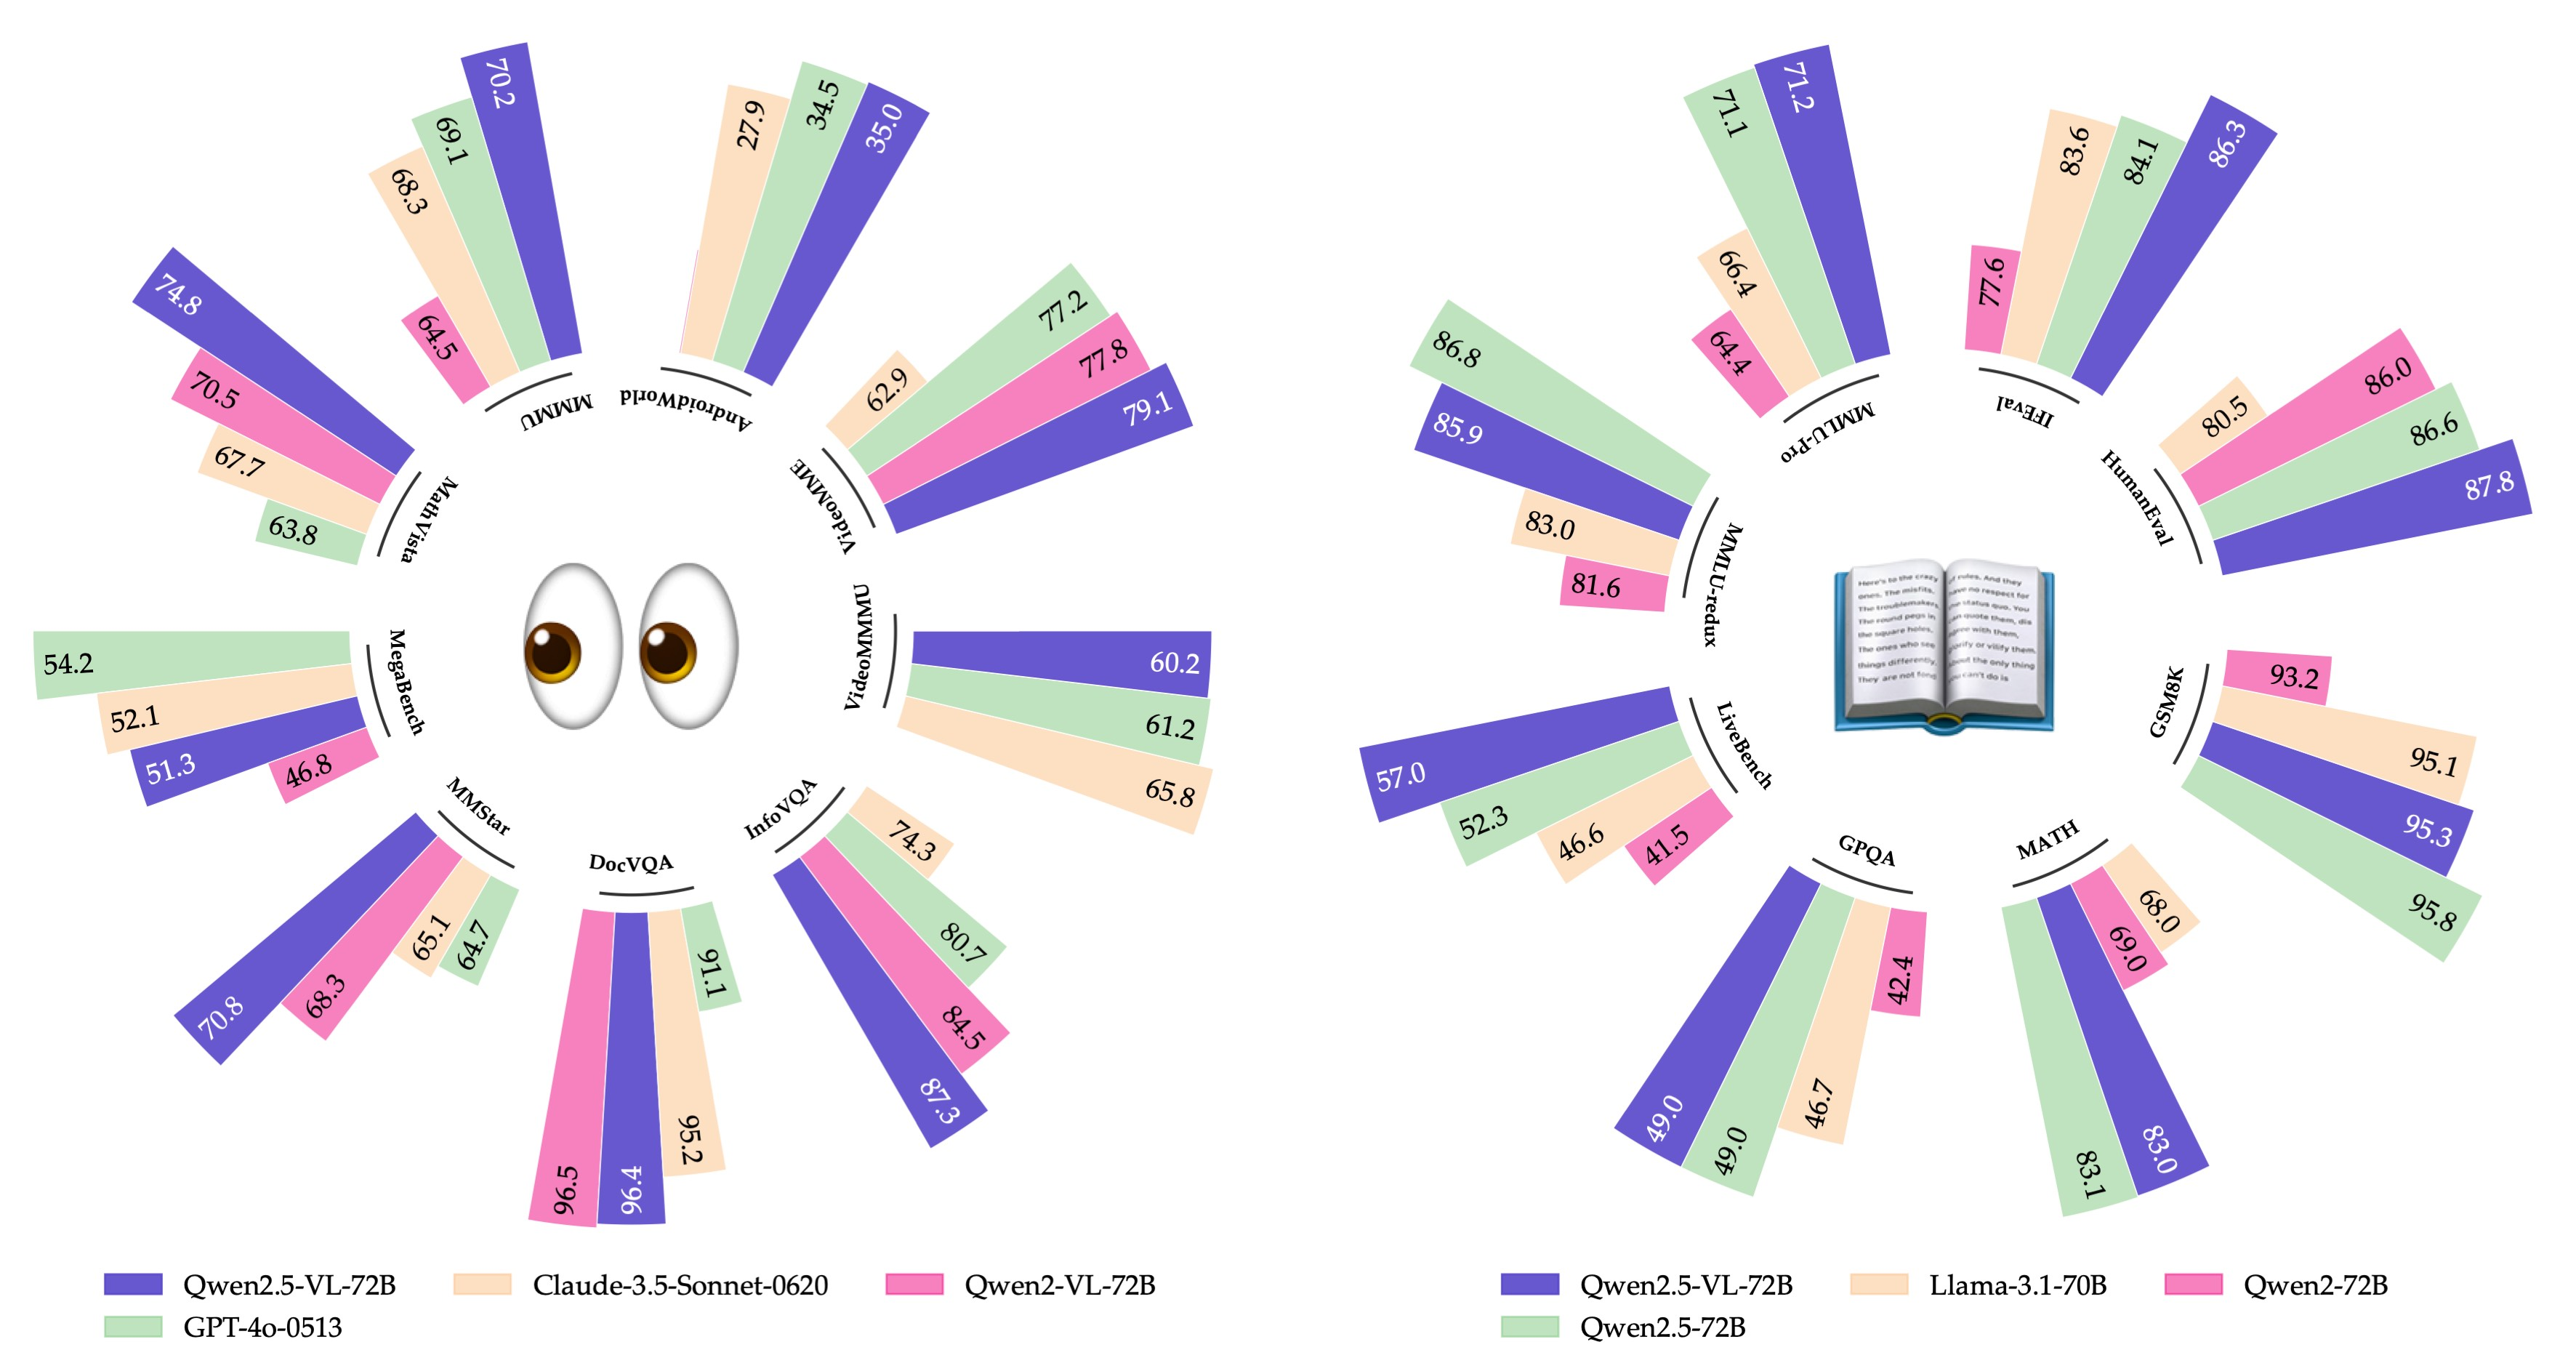
\includegraphics[width= 1\linewidth]{figures/head.jpg}
\end{figure*}

\section{Introduction}
%the development background of Qwen2.5-VL and highlights its latest advancements as a vision-language model, particularly focusing on breakthroughs in temporal and spatial awareness. It also outlines key features such as visual understanding, document parsing, video comprehension, object localization, and structured output generation.
Large vision-language models ( LVLMs )~\citep{gpt4o,sonnet3_5,team2023gemini,wang2024qwen2} represent a pivotal breakthrough in artificial intelligence, signaling a transformative approach to multimodal understanding and interaction. By seamlessly integrating visual perception with natural language processing, these advanced models are fundamentally reshaping how machines interpret and analyze complex information across diverse domains. Despite significant advancements in multimodal large language models, the current capabilities of these models can be likened to the middle layer of a sandwich cookie—competent across various tasks but falling short of exceptional performance. Fine-grained visual tasks form the foundational layer of this analogy. In this iteration of Qwen2.5-VL, we are committed to exploring fine-grained perception capabilities, aiming to establish a robust foundation for LVLMs and create an agentic amplifier for real-world applications. The top layer of this framework is multi-modal reasoning, which is enhanced by leveraging the latest Qwen2.5 LLM and employing multi-modal QA data construction.

% related work 
A spectrum of works have promoted the development of multimodal large models, characterized by architectural design, visual input processing, and data curation. One of the primary drivers of progress in LVLMs is the continuous innovation in architecture. The studies presented in~\citep{flamingo, blip, blip2, llava, llava1.5, wang2024emu3, zhang2024internlm,wang2023internimage} have incrementally shaped the current paradigm, which typically consists of a visual encoder, a cross-modal projector, and LLM. Fine-grained perception models have emerged as another crucial area. Models like ~\citep{xiao2023florence,grounding_dino,ren2024grounding, ferretv2,zhang2024omg,kosmos2,deitke2024molmo} have pushed the boundaries of what is possible in terms of detailed visual understanding. The architectures of Omni~\citep{li2024baichuan,li2025baichuan,ye2024x} and MoE~\citep{riquelme2021scaling,lee2024moai,li2024uni,li2024aria,wu2024deepseek} also inspire the future evolution of LVLMs. Enhancements in visual encoders~\citep{internvl, liu2024points,liang2025global} and resolution scaling~\citep{monkey,mplug-owl2,Otterhd} have played a pivotal role in improving the quality of practical visual understanding. Curating data with more diverse scenarios and higher-quality is an essential step in training advanced LVLMs. The efforts proposed in~\citep{guo2024mammoth,chen2024expanding, liu2024mminstruct, chen2024allava, tong2024cambrian, li2024llava} are highly valuable contributions to this endeavor. 

% the limitations of Current LVLMs
However, despite their remarkable progress, vision-language models currently face developmental bottlenecks, including computational complexity,  limited contextual understanding, poor fine-grained visual perception, and inconsistent performance across varied sequence length.

% \begin{figure*}[t]
% \centering
% 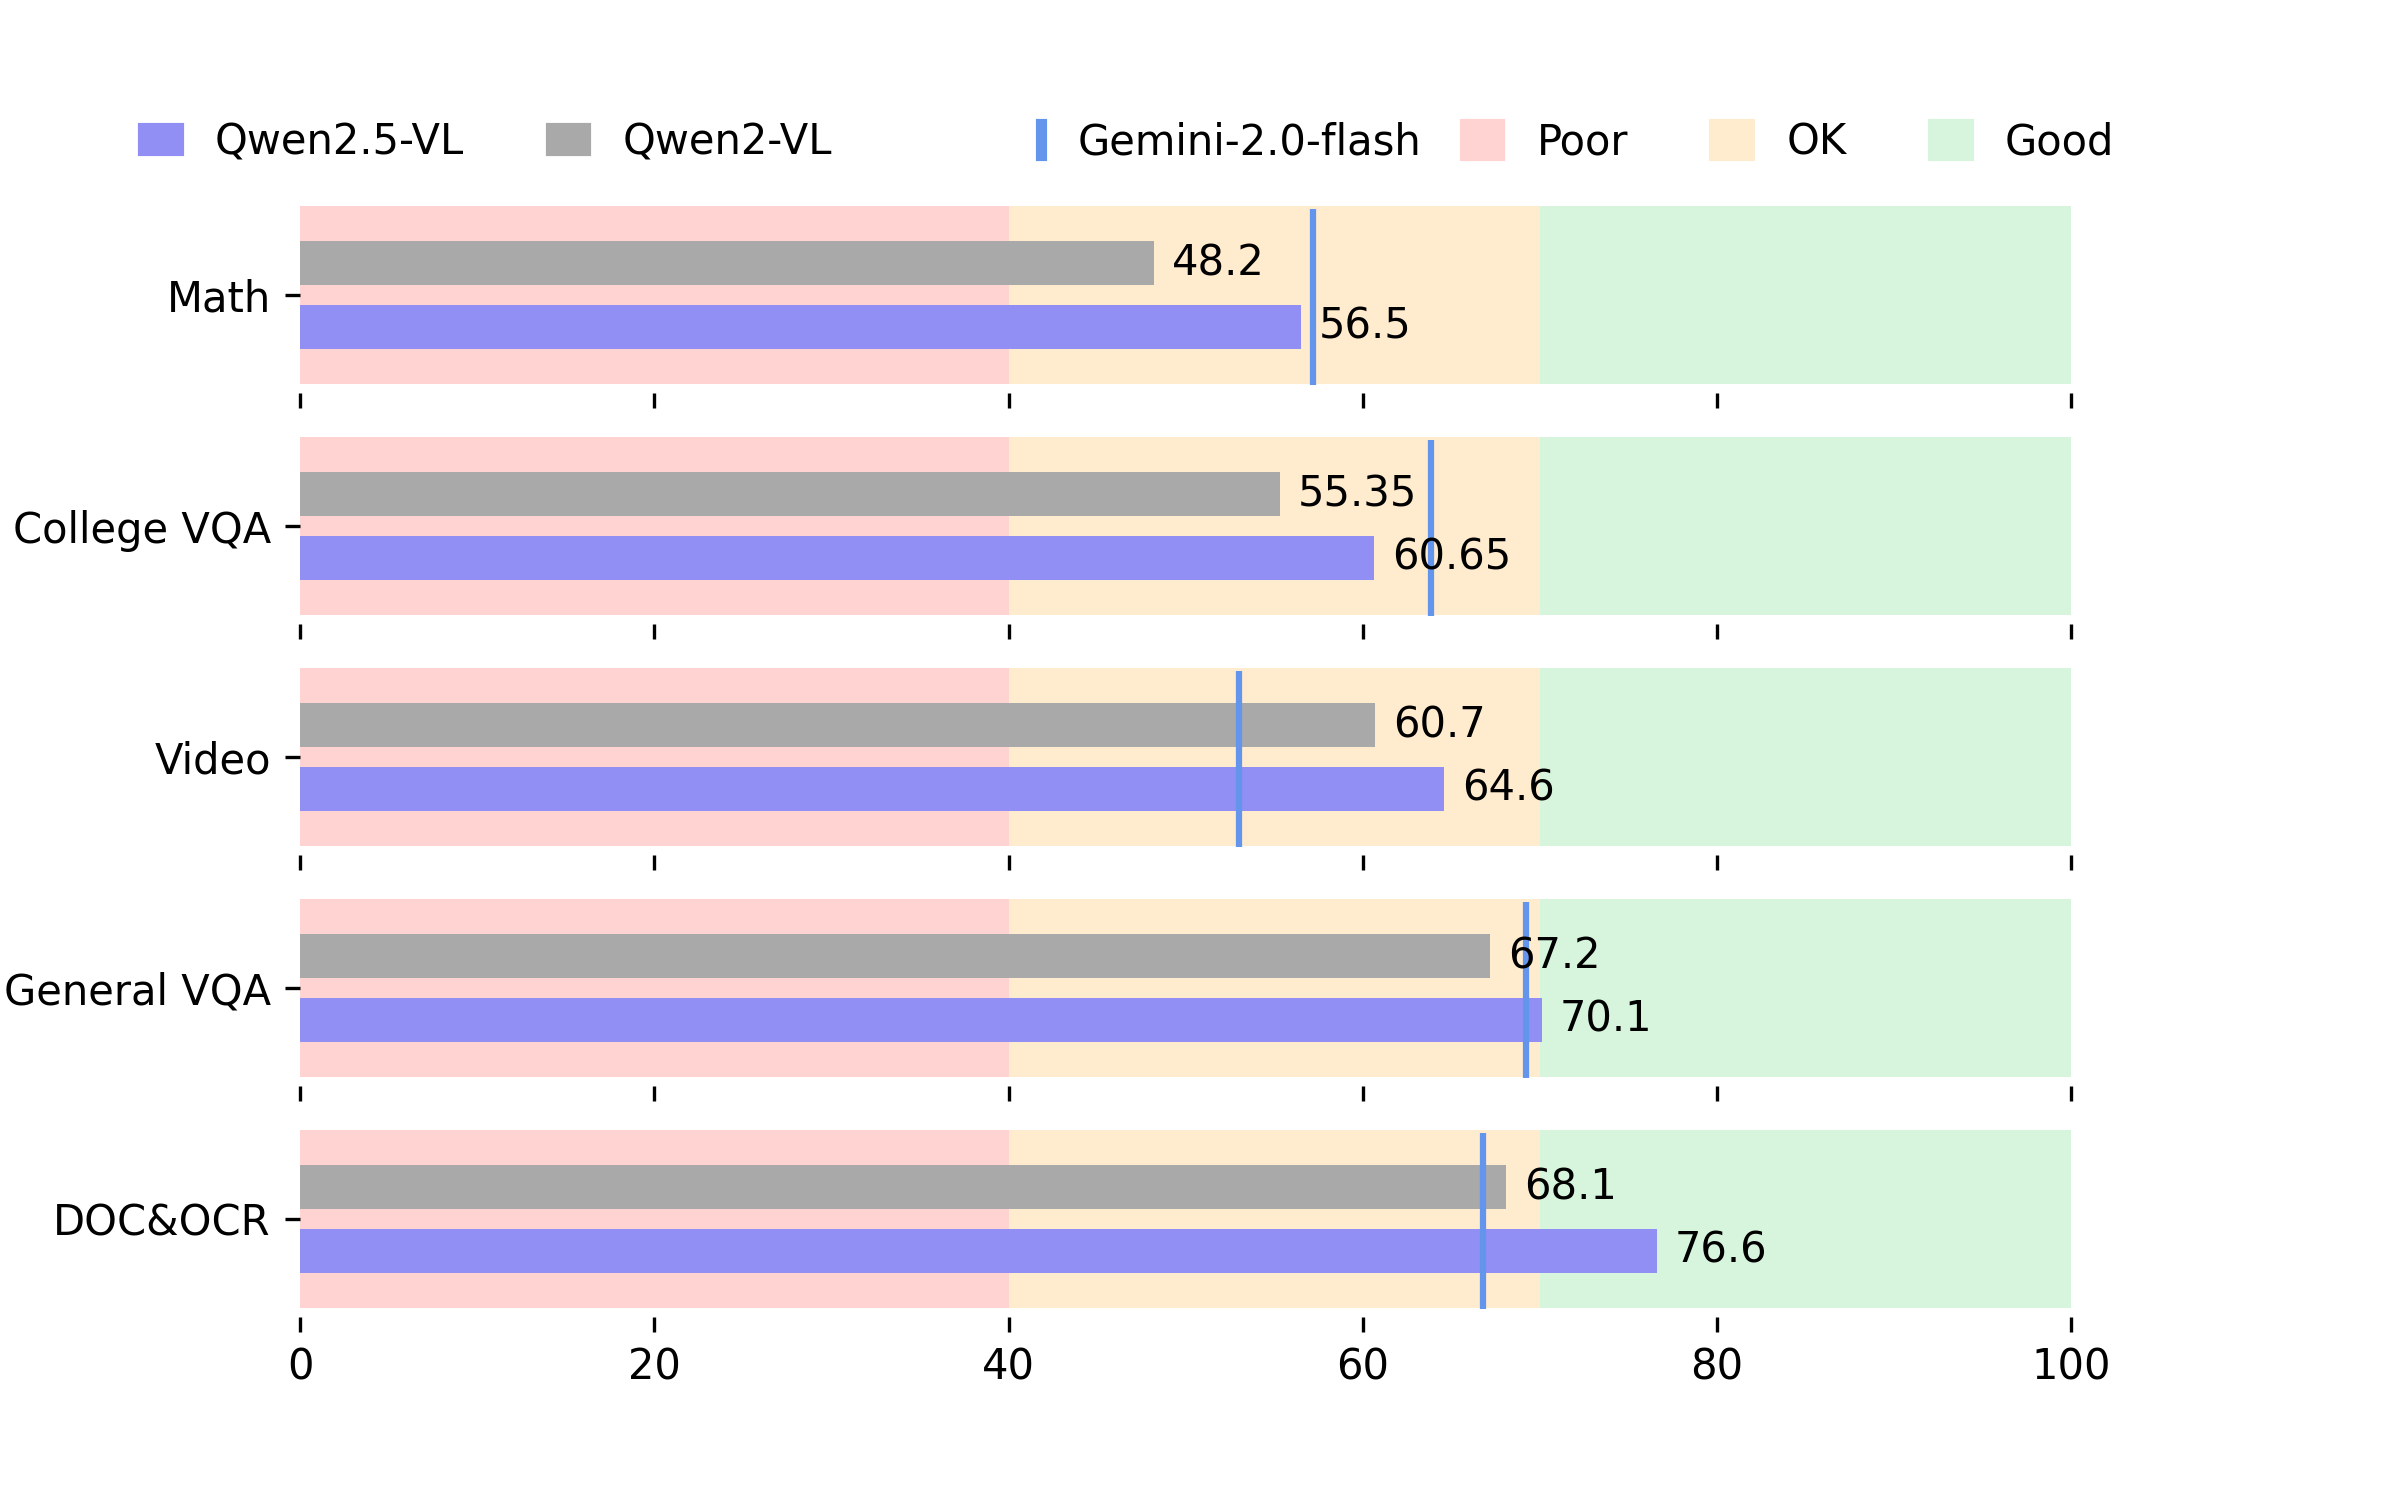
\includegraphics[width= 1\linewidth]{figures/bullet_introduction.png}
% \vspace{-10mm}
% \caption{Bullet Chart Comparison of the Qwen Series Models with Reference to Closed SOTA. Math ( MathVsita, MATH-Vsision ), College VQA ( MMMU, MMMU-PRO), Video ( Video-MME,MVBench, MMBench-Video, LVBench ), General VQA ( MMBench1.1, MegaBench, MMStar ), DOC\&OCR ( OCRBenchV1, OCRBenchV2, CC-OCR ). }
% \label{fig:intro}
% \end{figure*}
%the introduction of Qwen-vl
In this report, we introduce the latest work Qwen2.5-VL, which continues the open-source philosophy of the Qwen series, achieving and even surpassing top-tier closed-source models on various benchmarks. Technically, our contributions are four-folds: (1) We implement window attention in the visual encoder to optimize inference efficiency; (2) We introduce dynamic FPS sampling, extending dynamic resolution to the temporal dimension and enabling comprehensive video understanding across varied sampling rates; (3) We upgrade MRoPE in the temporal domain by aligning to absolute time, thereby facilitating more sophisticated temporal sequence learning; (4) We make significant efforts in curating high-quality data for both pre-training and supervised fine-tuning, further scaling the pre-training corpus from 1.2 trillion tokens to 4.1 trillion tokens.

%features
The sparkling characteristics of Qwen2.5-VL are as follows:
\begin{itemize}

 \item \textbf{Powerful document parsing capabilities:} Qwen2.5-VL upgrades text recognition to omni-document parsing, excelling in processing multi-scene, multilingual, and various built-in (handwriting, tables, charts, chemical formulas, and music sheets) documents.
 
 \item \textbf{Precise object grounding across formats:} Qwen2.5-VL unlocks improved accuracy in detecting, pointing, and counting objects, accommodating absolute coordinate and JSON formats for advanced spatial reasoning.
 
 \item \textbf{Ultra-long video understanding and fine-grained video grounding:} Our model extends native dynamic resolution to the temporal dimension, enhancing the ability to understand videos lasting hours while extracting event segments in seconds.
 
 \item \textbf{Enhanced agent Functionality for computer and mobile devices:} Leverage advanced grounding, reasoning, and decision-making abilities, boosting the model with superior agent functionality on smartphones and computers.
 
\end{itemize}

\section{Approach}

In this section, we first outline the architectural updates of the Qwen2.5-VL series models and provide an overview of the data and training details. 
% The Qwen2.5-VL series comprises three model variants with parameter sizes of 4B, 8B, and 73B. To better align with the naming conventions of the underlying Qwen large language models (LLMs), the models in the Qwen2.5-VL series are named according to the parameter counts of their corresponding LLMs. Thus, the series includes Qwen2.5-VL-72B, Qwen2.5-VL-7B, and Qwen2.5-VL-3B. This naming approach ensures consistency and clarity in identifying the specific configurations of the vision-language models.

\begin{figure*}[t]
\centering
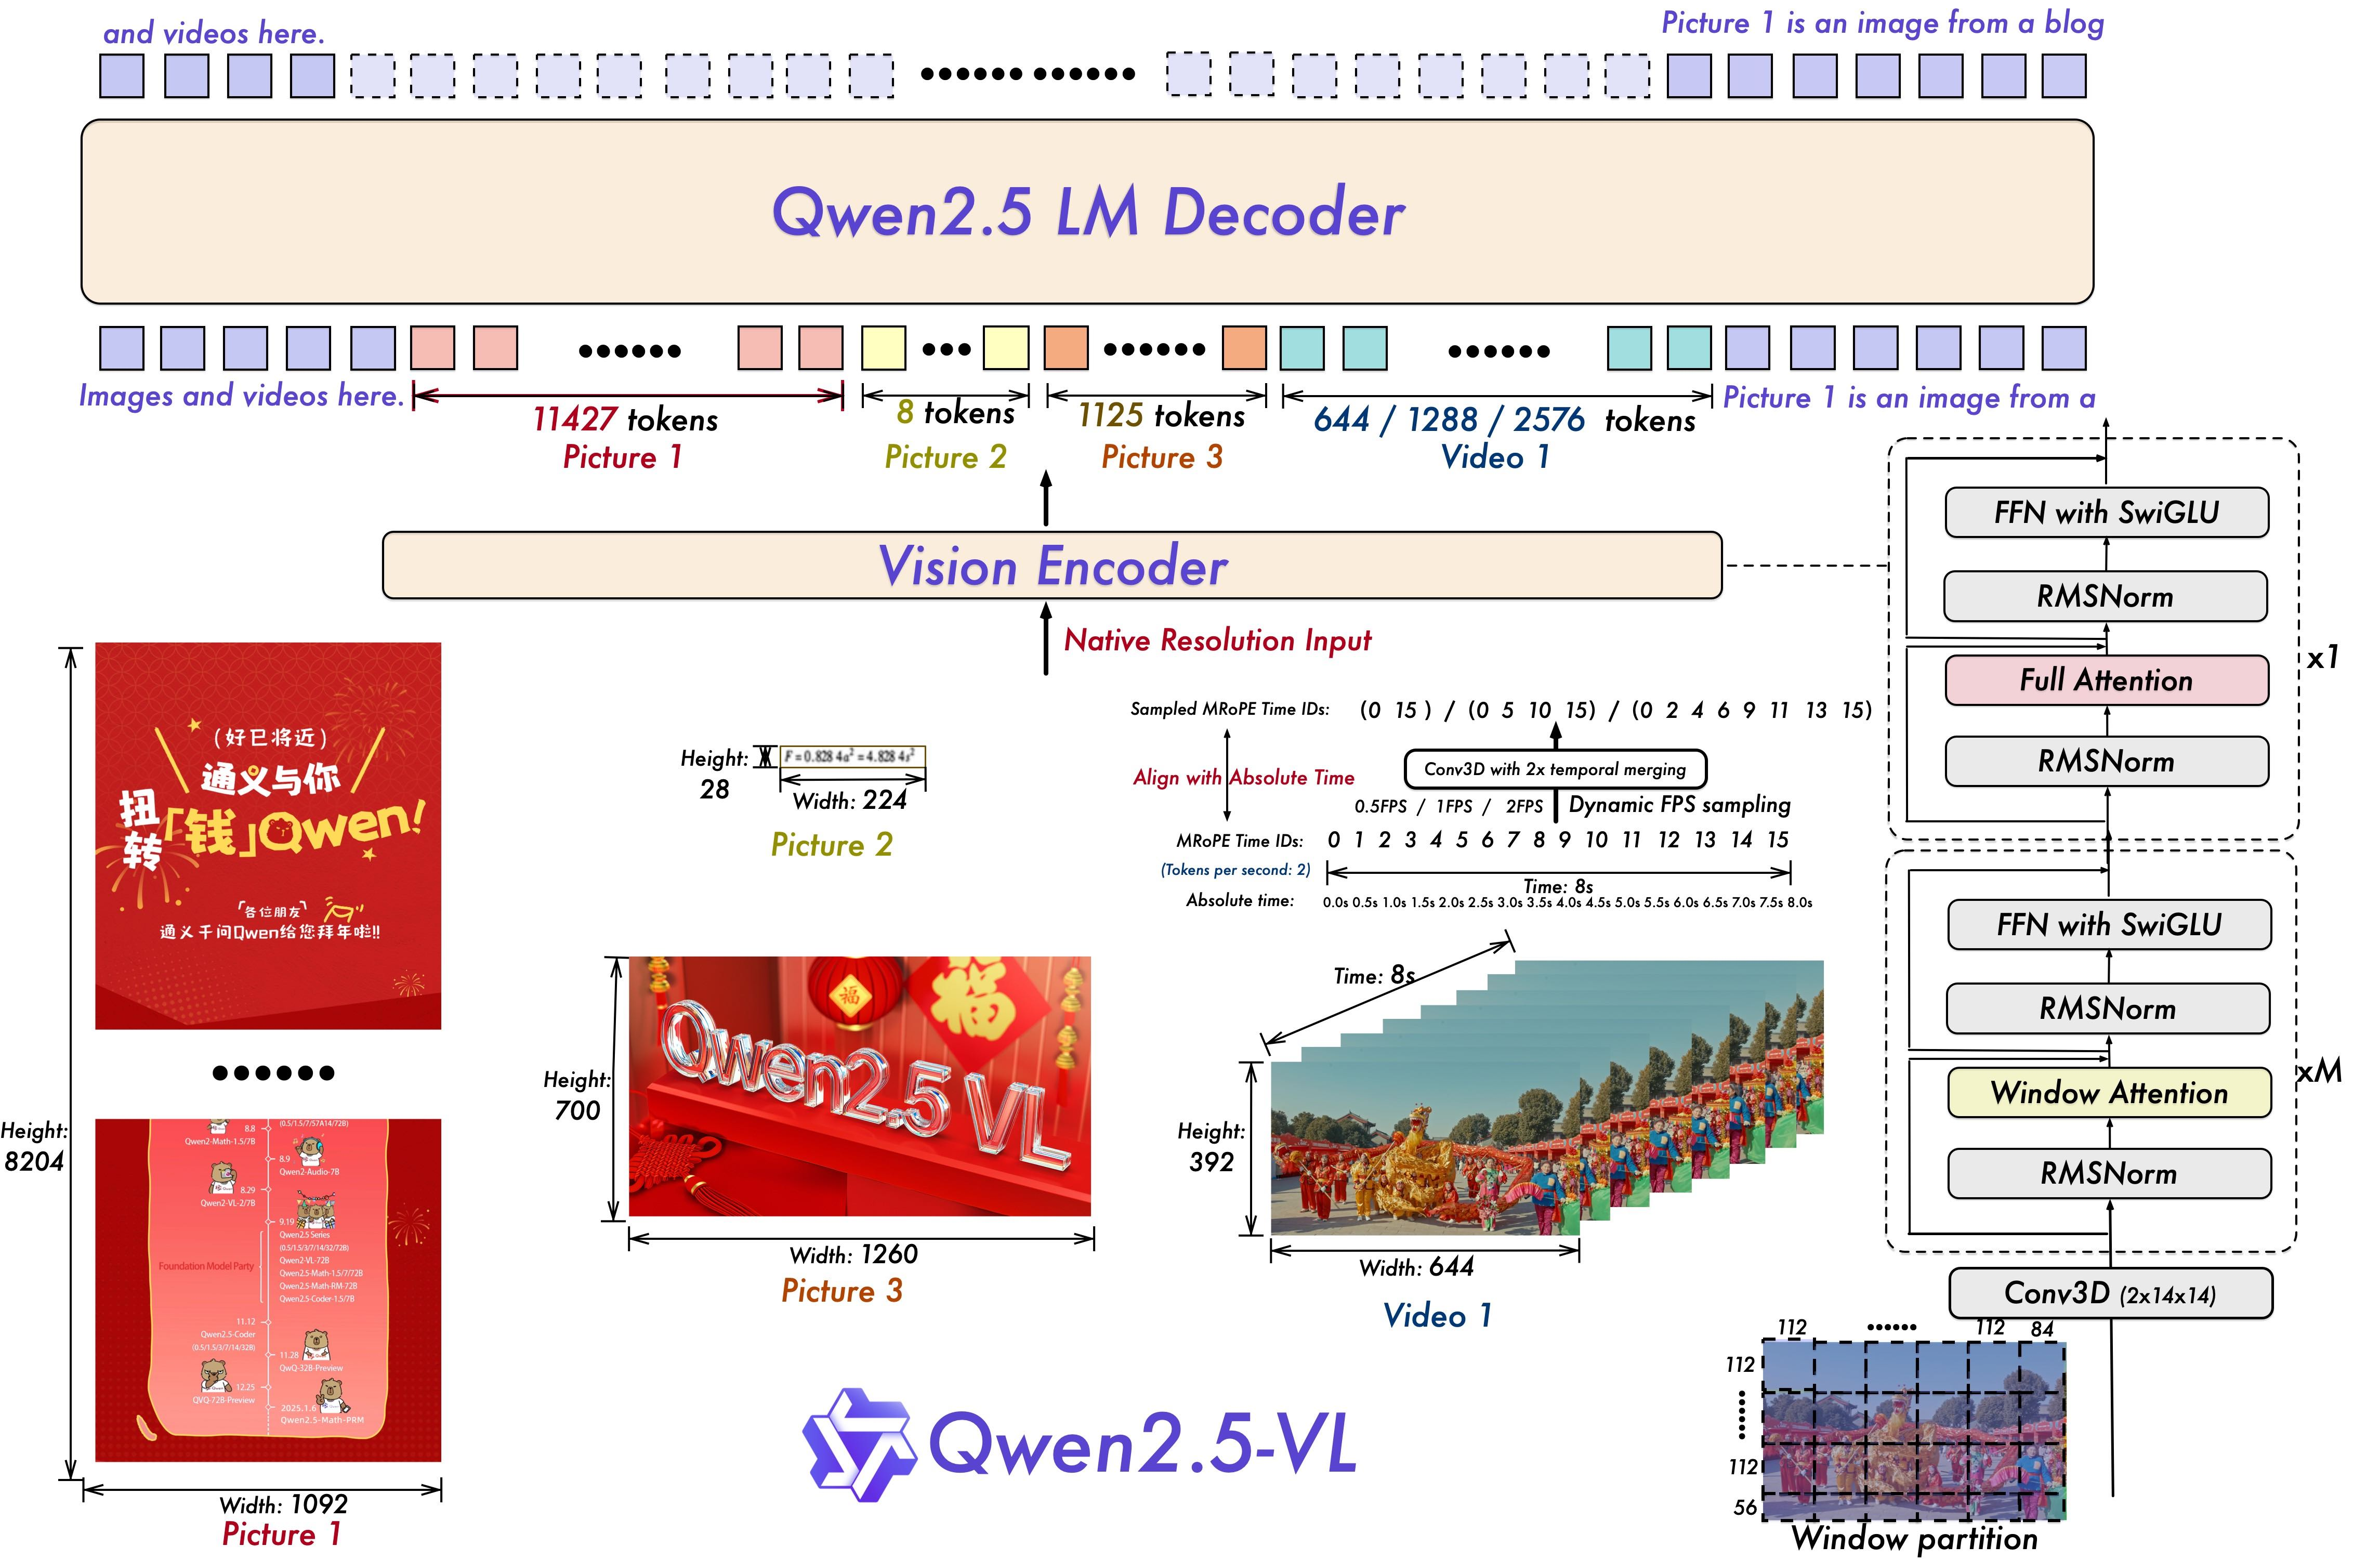
\includegraphics[width= 1\linewidth]{figures/qwen2.5vl_arc.jpeg}
   \caption{The Qwen2.5-VL framework demonstrates the integration of a vision encoder and a language model decoder to process multimodal inputs, including images and videos. The vision encoder is designed to handle inputs at their native resolution and supports dynamic FPS sampling. Images of varying sizes and video frames with different FPS rates are dynamically mapped to token sequences of varying lengths. Notably, MRoPE aligns time IDs with absolute time along the temporal dimension, enabling the model to better comprehend temporal dynamics, such as the pace of events and precise moment localization. The processed visual data is subsequently fed into the Qwen2.5 LM Decoder. We have re-engineered the vision transformer (ViT) architecture, incorporating advanced components such as FFN with SwiGLU activation, RMSNorm for normalization, and window-based attention mechanisms to enhance performance and efficiency.
}
\label{fig:arc}
\end{figure*}


\subsection{Model Architecture}
The overall model architecture of Qwen2.5-VL consists of three components:

\textbf{Large Language Model}: The Qwen2.5-VL series adopts large language models as its foundational component. The model is initialized with pre-trained weights from the Qwen2.5 LLM. To better meet the demands of multimodal understanding, we have modified the 1D RoPE (Rotary Position Embedding) to our Multimodal Rotary Position Embedding Aligned to Absolute Time.

\textbf{Vision Encoder}: The vision encoder of Qwen2.5-VL employs a redesigned Vision Transformer (ViT) architecture. Structurally, we incorporate 2D-RoPE and window attention to support native input resolutions while accelerating the computation of the entire visual encoder. During both training and inference, the height and width of the input images are resized to multiples of 28 before being fed into the ViT. The vision encoder processes images by splitting them into patches with a stride of 14, generating a set of image features. We provide a more detailed introduction to the vision encoder in Section~\ref{sec:VisionEncoder}.

\textbf{MLP-based Vision-Language Merger}: To address the efficiency challenges posed by long sequences of image features, we adopt a simple yet effective approach to compress the feature sequences before feeding them into the large language model (LLM). Specifically, instead of directly using the raw patch features extracted by the Vision Transformer (ViT), we first group spatially adjacent sets of four patch features. These grouped features are then concatenated and passed through a two-layer multi-layer perceptron (MLP) to project them into a dimension that aligns with the text embeddings used in the LLM. This method not only reduces computational costs but also provides a flexible way to dynamically compress image feature sequences of varying lengths.

In Table~\ref{table:config}, the architecture and configuration of Qwen2.5-VL are detailed.

\begin{table}[htbp]
\centering
\begin{tabular}{lccc}
\toprule
\textbf{Configuration} & \textbf{Qwen2.5-VL-3B} & \textbf{Qwen2.5-VL-7B} & \textbf{Qwen2.5-VL-72B} \\ \midrule
\multicolumn{4}{c}{\textbf{Vision Transformer (ViT) }} \\ \midrule
Hidden Size & 1280 & 1280 & 1280 \\
\# Layers & 32 & 32 & 32 \\
\# Num Heads & 16 & 16 & 16 \\
Intermediate Size & 3456 & 3456 & 3456 \\
Patch Size & 14 & 14 & 14 \\
Window Size & 112 & 112 & 112 \\
Full Attention Block Indexes & \{7, 15, 23, 31\} & \{7, 15, 23, 31\} & \{7, 15, 23, 31\} \\ \midrule
\multicolumn{4}{c}{\textbf{Vision-Language Merger}} \\  \midrule
In Channel & 1280 & 1280 & 1280 \\
Out Channel & 2048 & 3584 & 8192 \\ \midrule
\multicolumn{4}{c}{\textbf{Large Language Model (LLM) }} \\ \midrule
Hidden Size & 2048 & 3,584 & 8192 \\
\# Layers & 36 & 28 & 80 \\
\# KV Heads & 2 & 4 & 8 \\
Head Size & 128 & 128 & 128 \\
Intermediate Size & 4864 & 18944 & 29568 \\
Embedding Tying & \ding{51} & \ding{55} & \ding{55} \\
Vocabulary Size & 151646 & 151646 & 151646 \\
\# Trained Tokens & 4.1T & 4.1T & 4.1T \\ 

\bottomrule
\end{tabular}
\caption{Configuration of Qwen2.5-VL.}
\label{table:config}
\end{table}



\subsubsection{Fast and Efficient Vision Encoder}
\label{sec:VisionEncoder}

The vision encoder plays a pivotal role in multimodal large language models (MLLMs). To address the challenges posed by computational load imbalances during training and inference due to native resolution inputs, we have redesigned the Vision Transformer (ViT) architecture. A key issue arises from the quadratic computational complexity associated with processing images of varying sizes. To mitigate this, we introduce windowed attention in most layers, which ensures that computational cost scales linearly with the number of patches rather than quadratically. In our architecture, only four layers employ full self-attention, while the remaining layers utilize windowed attention with a maximum window size of 112×112 (corresponding to 8×8 patches). Regions smaller than 112×112 are processed without padding, preserving their original resolution. This design allows the model to operate natively at the input resolution, avoiding unnecessary scaling or distortion.

For positional encoding, we adopt 2D Rotary Positional Embedding (RoPE) to effectively capture spatial relationships in 2D space. Furthermore, to better handle video inputs, we extend our approach to 3D patch partitioning. Specifically, we use 14×14 image patches as the basic unit, consistent with traditional ViTs for static images. For video data, two consecutive frames are grouped together, significantly reducing the number of tokens fed into the language model. This design not only maintains compatibility with existing architectures but also enhances efficiency when processing sequential video data.

To streamline the overall network structure, we align the ViT architecture more closely with the design principles of large language models (LLMs). Specifically, we adopt RMSNorm~\citep{rmsnorm} for normalization and SwiGLU~\citep{glu} as the activation function. These choices enhance both computational efficiency and compatibility between the vision and language components of the model.

In terms of training, we train the redesigned ViT from scratch. The training process consists of several stages, including CLIP pre-training, vision-language alignment, and end-to-end fine-tuning. To ensure robustness across varying input resolutions, we employ dynamic sampling at native resolutions during training. Images are randomly sampled according to their original aspect ratios, enabling the model to generalize effectively to inputs of diverse resolutions. This approach not only improves the model's adaptability but also ensures stable and efficient training across different sizes of visual data. 

\subsubsection{Native Dynamic Resolution and Frame Rate}

Qwen2.5-VL introduces advancements in both spatial and temporal dimensions to handle diverse multimodal inputs effectively.

In the spatial domain, Qwen2.5-VL dynamically converts images of varying sizes into sequences of tokens with corresponding lengths. Unlike traditional approaches that normalize coordinates, our model directly uses the actual dimensions of the input image to represent bounding boxes, points, and other spatial features. This allows the model to learn scale information inherently, improving its ability to process images across different resolutions.

For video inputs, Qwen2.5-VL incorporates dynamic frame rate (FPS) training and absolute time encoding. By adapting to variable frame rates, the model can better capture the temporal dynamics of video content.
Unlike other approaches that incorporate textual timestamps or utilize additional heads to enable temporal grounding, we introduce a novel and efficient strategy that aligns MRoPE IDs directly with the timestamps. This approach allows the model to understand the tempo of time through the intervals between temporal dimension IDs, without necessitating any additional computational overhead.
% Absolute time encoding provides the model with precise timing information, enabling it to reason about events occurring at specific moments within a video sequence.


\subsubsection{Multimodal Rotary Position Embedding Aligned to Absolute Time}

Positional embeddings are crucial for modeling sequential data in both vision and language modalities. Building upon the Multimodal Rotary Position Embedding (MRoPE) introduced in Qwen2-VL, we extend its capabilities to better handle temporal information in videos.

The MRoPE in Qwen2-VL decomposes the position embedding into three distinct components: temporal, height, and width to effectively model multimodal inputs. For textual inputs, all three components use identical position IDs, making MRoPE functionally equivalent to traditional 1D RoPE~\citep{rope}. For images, the temporal ID remains constant across visual tokens, while unique IDs are assigned to the height and width components based on each token's spatial position within the image. When processing videos, which are treated as sequences of frames, the temporal ID increments for each frame, while the height and width components follow the same assignment pattern as for static images.

However, in Qwen2-VL, the temporal position IDs in MRoPE were tied to the number of input frames, which did not account for the speed of content changes or the absolute timing of events within the video. To address this limitation, Qwen2.5-VL introduces a key improvement: aligning the temporal component of MRoPE with absolute time. As shown in Figure~\ref{fig:arc}, by leveraging the intervals between temporal IDs, the model is able to learn consistent temporal alignment across videos with different FPS sampling rates.


\subsection{Pre-Training}
In this section, we first describe the construction of the pre-training dataset, followed by an overview of the overall training pipeline and configuration.
\subsubsection{Pre-Training Data}
Compared to Qwen2-VL, we have significantly expanded the volume of our pre-training data, increasing it from 1.2 trillion tokens to approximately 4 trillion tokens. Our pre-training dataset was constructed through a combination of methods, including cleaning raw web data, synthesizing data, etc. The dataset encompasses a wide variety of multimodal data, such as image captions, interleaved image-text data, optical character recognition (OCR) data, visual knowledge (e.g., celebrity, landmark, flora, and fauna identification), multi-modal academic questions, localization data, document parsing data, video descriptions, video localization, and agent-based interaction data. Throughout the training process, we carefully adjusted the composition and proportions of these data types at different stages to optimize learning outcomes.





\paragraph{Interleaved Image-Text Data}
Interleaved image-text data is essential for multimodal learning, offering three key benefits: (1) enabling in-context learning with simultaneous visual and textual cues~\citep{flamingo}, (2) maintaining strong text-only capabilities when images are missing~\citep{lin2024vila}, and (3) containing a wide range of general information. However, much of the available interleaved data lacks meaningful text-image associations and is often noisy, limiting its usefulness for complex reasoning and creative generation.

To address these challenges, we developed a pipeline for scoring and cleaning data, ensuring only high-quality, relevant interleaved data is used. Our process involves two steps: standard data cleaning~\citep{li2024omnicorpus} followed by a four-stage scoring system using an internal evaluation model. The scoring criteria include: (1) text-only quality, (2) image-text relevance, (3) image-text complementarity, and (4) information density balance. This meticulous approach improves the model’s ability to perform complex reasoning and generate coherent multimodal content.

The following is a description of these image-text scoring criteria:

Image-text Relevance: A higher score indicates a stronger connection between the image and text, where the image meaningfully supplements, explains or expands on the text rather than just decorating it.

Information Complementarity: A higher score reflects greater complementary information between the image and text. Each should provide unique details that together create a complete narrative.

Balance of Information Density: A higher score means a more balanced distribution of information between the image and text, avoiding excessive text or image information, and ensuring an appropriate balance between the two.


\paragraph{Grounding Data with Absolute Position Coordinates}
We adopt native resolution training with the aim of achieving a more accurate perception of the world. In contrast, relative coordinates fail to effectively represent the original size and position of objects within images. To address this limitation, Qwen2.5-VL uses coordinate values based on the actual dimensions of the input images during training to represent bounding boxes and points. This approach ensures that the model can better capture the real-world scale and spatial relationships of objects, leading to improved performance in tasks such as object detection and localization.

%data format and pipeline
To improve the generalizability of grounding capabilities, we have developed a comprehensive dataset encompassing bounding boxes and points with referring expressions, leveraging both publicly available datasets and proprietary data. 
Our methodology involves synthesizing data into various formats, including XML, JSON, and custom formats, employing techniques such as copy-paste augmentation~\citep{ghiasi2021simple} and synthesis with off-the-shelf models such as Grounding DINO~\citep{grounding_dino} and SAM~\citep{kirillov2023segment}. This approach facilitates a more robust evaluation and advancement of grounding abilities.

To enhance the model's performance on open-vocabulary detection, we expanded the training dataset to include over 10,000 object categories. Additionally, to improve the model's effectiveness in extreme object detection scenarios, we synthesized non-existent object categories within the queries and constructed image data containing multiple instances for each object.

% bboxing box data
%point data
To ensure superior point-based object grounding capabilities, we have constructed a comprehensive pointing dataset comprising both publicly available and synthetic data. Specifically, the data source includes public pointing and counting data from PixMo~\citep{deitke2024molmo}, publicly accessible object grounding data (from both object detection and instance segmentation tasks), and data synthesized by an automated pipeline for generating precise pointing data towards certain image details.

\paragraph{Document Omni-Parsing Data}
To train Qwen2.5-VL, we synthesized a large corpus of document data. Traditional methods for parsing document content typically rely on separate models to handle layout analysis, text extraction, chart interpretation, and illustration processing. In contrast, Qwen2.5-VL is designed to empower a general-purpose model with comprehensive capabilities for parsing, understanding, and converting document formats. Specifically, we incorporated a diverse array of elements into the documents, such as tables, charts, equations, natural or synthetic images, music sheets, and chemical formulas. These elements were uniformly formatted in HTML, which integrates layout box information and descriptions of illustrations into HTML tag structures. We also enriched the document layouts according to typical reading sequences and included the coordinates corresponding to each module, such as paragraphs and charts, in the HTML-based ground truth. This innovative approach allows the complete information of any document, including its layout, text, charts, and illustrations, to be represented in a standardized and unified manner. As a result, Qwen2.5-VL achieves seamless integration of multimodal document elements, thereby facilitating more efficient and accurate document understanding and transformation.

Below is the QwenVL HTML format:

\begin{tcolorbox}[colback=black!5!white,colframe=black!75!black,title=QwenVL HTML Format]
<html><body> \\
\textcolor{blue}{\# paragraph} \\
<p data-bbox="\textcolor{red}{x1 y1 x2 y2}"> \textcolor{red}{content} </p> \\
\textcolor{blue}{\# table} \\
<style>\textcolor{red}{table\{id\} style}</style><table data-bbox="\textcolor{red}{x1 y1 x2 y2}" class="table\textcolor{red}{\{id\}}"> \textcolor{red}{table content} </table> \\
\textcolor{blue}{\# chart} \\
<div class="chart" data-bbox="\textcolor{red}{x1 y1 x2 y2}"> <img data-bbox="\textcolor{red}{x1 y1 x2 y2}" /><table> \textcolor{red}{chart content} </table></div> \\
\textcolor{blue}{\# formula} \\
<div class="formula" data-bbox="\textcolor{red}{x1 y1 x2 y2}"> <img data-bbox="\textcolor{red}{x1 y1 x2 y2}" /> <div> \textcolor{red}{formula content} </div></div>\\
\textcolor{blue}{\# image caption} \\
<div class="image caption" data-bbox="\textcolor{red}{x1 y1 x2 y2}"> <img data-bbox="\textcolor{red}{x1 y1 x2 y2}" /><p> \textcolor{red}{image caption} </p></div>\\
\textcolor{blue}{\# image ocr} \\
<div class="image ocr" data-bbox="\textcolor{red}{x1 y1 x2 y2}"> <img data-bbox="\textcolor{red}{x1 y1 x2 y2}" /><p> \textcolor{red}{image ocr} </p></div>\\
\textcolor{blue}{\# music sheet} \\
<div class="music sheet" format="abc notation" data-bbox="\textcolor{red}{x1 y1 x2 y2}"> <img data-bbox="\textcolor{red}{x1 y1 x2 y2}" /> <div> \textcolor{red}{music sheet content} </div></div> \\
\textcolor{blue}{\# chemical formula content} \\
<div class="chemical formula" format="smile" data-bbox="\textcolor{red}{x1 y1 x2 y2}"> <img data-bbox="\textcolor{red}{x1 y1 x2 y2}" /> <div> \textcolor{red}{chemical formula content} </div></div> \\
</html></body>
\end{tcolorbox}

This format ensures that all document elements are represented in a structured and accessible manner, enabling efficient processing and understanding by Qwen2.5-VL.


\paragraph{OCR Data} Data from different sources are gathered and curated to enhance the OCR performance, including synthetic data, open-sourced data and in-house collected data. Synthetic data is generated through a visual text generation engine to produce high-quality text images in the wild. To support a wider range of languages and enhance multilingual capabilities, we have incorporated a large-scale multilingual OCR dataset. This dataset includes support for diverse languages such as French, German, Italian, Spanish, Portuguese, Arabic, Russian, Japanese, Korean, and Vietnamese. The dataset is carefully curated to ensure diversity and quality, utilizing both high-quality synthetic images and real-world natural scene images. This combination ensures robust performance across various linguistic contexts and improves the model’s adaptability to different text appearances and environmental conditions. For chart-type data, we synthesized 1 million samples using visualization libraries including matplotlib, seaborn, and plotly, encompassing chart categories such as bar charts, relational diagrams, and heatmaps. Regarding tabular data, we processed 6 million real-world samples through an offline end-to-end table recognition model, subsequently filtering out low-confidence tables, overlapping tables, and tables with insufficient cell density.

\paragraph{Video Data}
To ensure enhanced robustness in understanding video data with varying frames per second (FPS), we dynamically sampled FPS during training to achieve a more evenly distributed representation of FPS within the training dataset. Additionally, for videos exceeding half an hour in length, we specifically constructed a set of long video captions by synthesizing multi-frame captions through a targeted synthesis pipeline. Regarding video grounding data, we formulated timestamps in both second-based formats and hour-minute-second-frame (hmsf) formats, ensuring that the model can accurately understand and output time in various formats.

\paragraph{Agent Data}

We enhance the perception and decision-making abilities to build the agent capabilities of Qwen2.5-VL. For perception, we collect screenshots on mobile, web, and desktop platforms. A synthetic data engine is used to generate screenshot captions and UI element grounding annotations. The caption task helps Qwen2.5-VL understand the graphic interface, while the grounding task helps it align the appearance and function of elements. For decision-making, we first unify the operations across mobile, web, and desktop platforms into a function call format with a shared action space. A set of annotated multi-step trajectories collected from open-source data and synthesized by agent framework~\citep{wang2025mobile, wang2024mobile2, wang2024mobile} on virtual environments are reformatted into a function format. We further generate a reasoning process for each step through human and model annotators~\citep{xu2024aguvis}. Specifically, given a ground-truth operation, we highlight it on the screenshot. Then, we provide the global query, along with screenshots from before and after this operation, to the annotators and require them to write reasoning content to explain the intention behind this operation. A model-based filter is used to screen out low-quality reasoning content. Such reasoning content prevents Qwen2.5-VL from overfitting to the ground-truth operations and makes it more robust in real-world scenarios.

\begin{table}[h!]
\small
\centering
\begin{tabular}{lccc}
\toprule
\textbf{Stages}        & \textbf{Visual Pre-Training}       & \textbf{Multimodal Pre-Training}       & \textbf{Long-Context Pre-Training}       \\ \midrule
Data   &   \makecell{Image Caption \\ Knowledge \\ OCR}     & \makecell{+ \\ Pure text \\ Interleaved Data \\ VQA, Video \\ Grounding, Agent}   &     \makecell{+ \\ 
 Long Video\\ Long Agent \\ Long Document}    \\ 
\midrule
Tokens&  1.5T  &    2T   &    0.6T   \\ 
\midrule
Sequence length   &  8192  &    8192   &    32768   \\ 
\midrule
Training   &  ViT  &    ViT \& LLM   &    ViT \& LLM   \\ 
\bottomrule
\end{tabular}
\caption{Training data volume and composition across different stages.}
\label{tab:pretrainingdata}
\end{table}


% 668m vit size
\subsubsection{Training Recipe}
We trained a Vision Transformer (ViT) from scratch using DataComp~\citep{datacomp} and some in-house datasets as the initialization for the vision encoder, while leveraging the pre-trained Qwen2.5 large language model (LLM)~\citep{qwen2.5} as the initialization for the LLM component. As shown in Table \ref{tab:pretrainingdata}, the pre-training process is divided into three distinct phases, each employing different data configurations and training strategies to progressively enhance the model's capabilities.

In the first phase, only the Vision Transformer (ViT) is trained to improve its alignment with the language model, laying a solid foundation for multimodal understanding. The primary data sources during this phase include image captions, visual knowledge, and OCR data. These datasets are carefully selected to foster ViT's ability to extract meaningful visual representations that can be effectively integrated with textual information.

In the second phase, all model parameters are unfrozen, and the model is trained on a diverse set of multimodal image data to enhance its capacity to process complex visual information. This phase introduces more intricate and reasoning-intensive datasets, such as interleaved data, multi-task learning datasets, visual question answering (VQA), multimodal mathematics, agent-based tasks, video understanding, and pure-text datasets. These datasets strengthen the model's ability to establish deeper connections between visual and linguistic modalities, enabling it to handle increasingly sophisticated tasks.

In the third phase, to further enhance the model's reasoning capabilities over longer sequences, video, and agent-based data are incorporated, alongside an increase in sequence length. This allows the model to tackle more advanced and intricate multimodal tasks with greater precision. By extending the sequence length, the model gains the ability to process extended contexts, which is particularly beneficial for tasks requiring long-range dependencies and complex reasoning.

To address the challenges posed by varying image sizes and text lengths, which can lead to imbalanced computational loads during training, we adopted a strategy to optimize training efficiency. The primary computational costs arise from the LLM and the vision encoder. Given that the vision encoder has relatively fewer parameters and that we introduced window attention to further reduce its computational demands, we focused on balancing the computational load of the LLM across different GPUs. Specifically, we dynamically packed data samples based on their corresponding input sequence lengths to the LLM, ensuring consistent computational loads. In the first and second phases, data were uniformly packed to a sequence length of 8,192, while in the third phase, the sequence length was increased to 32,768 to accommodate the model's enhanced capacity for handling longer sequences.

\subsection{Post-training}

The post-training alignment framework of Qwen2.5-VL employs a dual-stage optimization paradigm comprising Supervised Fine-Tuning (SFT) and Direct Preference Optimization (DPO)~\citep{DBLP:conf/nips/RafailovSMMEF23}. This hierarchical alignment strategy synergizes parameter-efficient domain adaptation with human preference distillation, addressing both representational grounding and behavioral refinement through distinct optimization objectives.

Supervised Fine-Tuning (SFT) aims to bridge the gap between pretrained representations and downstream task requirements through targeted instruction optimization. During this phase, we employ the ChatML format~\citep{chatml} to structure instruction-following data, deliberately diverging from the pretraining data schema while maintaining architectural consistency with Qwen2-VL~\citep{Qwen2-VL}. This format transition enables three critical adaptations: 1) Explicit dialogue role tagging for multimodal turn-taking, 2) Structured injection of visual embeddings alongside textual instructions, and 3) Preservation of cross-modal positional relationships through format-aware packing. By exposing the model to curated multimodal instruction-response pairs under this enhanced schema, SFT enables efficient knowledge transfer while maintaining the integrity of pre-trained features. 

\subsubsection{Instruction Data}

The Supervised Fine-Tuning (SFT) phase employs a meticulously curated dataset designed to enhance the model's instruction-following capabilities across diverse modalities. This dataset comprises approximately 2 million entries, evenly distributed between pure text data (50\%) and multimodal data (50\%), which includes image-text and video-text combinations. The inclusion of multimodal data enables the model to process complex inputs effectively. Notably, although pure text and multimodal entries are equally represented, multimodal entries consume significantly more tokens and computational resources during training due to the embedded visual and temporal information. The dataset is primarily composed of Chinese and English data, with supplementary multilingual entries to support broader linguistic diversity.

The dataset is structured to reflect varying levels of dialogue complexity, including both single-turn and multi-turn interactions. These interactions are further contextualized by scenarios ranging from single-image inputs to multi-image sequences, thereby simulating realistic conversational dynamics. The query sources are primarily drawn from open-source repositories, with additional contributions from curated purchased datasets and online query data. This combination ensures broad coverage and enhances the representativeness of the dataset.

To address a wide range of application scenarios, the dataset includes specialized subsets for General Visual Question Answering (VQA), image captioning, mathematical problem-solving, coding tasks, and security-related queries. Additionally, dedicated datasets for Document and Optical Character Recognition (Doc and OCR), Grounding, Video Analysis, and Agent Interactions are constructed to enhance domain-specific proficiency. Detailed information regarding the data can be found in the relevant sections of the paper. This structured and diverse composition ensures that the SFT phase effectively aligns pre-trained representations with the nuanced demands of downstream multimodal tasks, fostering robust and contextually aware model performance.


\subsubsection{Data Filtering Pipeline}

The quality of training data is a critical factor influencing the performance of vision-language models. Open-source and synthetic datasets typically exhibit significant variability, often containing noisy, redundant, or low-quality samples. Therefore, rigorous data cleaning and filtering processes are essential to address these issues. Low-quality data can lead to suboptimal alignment between pretrained representations and downstream task requirements, thereby diminishing the model's ability to effectively handle complex multimodal tasks. Consequently, ensuring high-quality data is paramount for achieving robust and reliable model performance.

To address these challenges, we implement a two-stage data filtering pipeline designed to systematically enhance the quality of the Supervised Fine-Tuning (SFT) dataset. This pipeline comprises the following stages:

\paragraph{Stage 1: Domain-Specific Categorization}

In the initial stage, we employ \textit{Qwen2-VL-Instag}, a specialized classification model derived from Qwen2-VL-72B, to perform hierarchical categorization of question-answer (QA) pairs. This model organizes QA pairs into eight primary domains, such as \textit{Coding} and \textit{Planning}, which are further divided into 30 fine-grained subcategories. For example, the primary domain \textit{Coding} is subdivided into subcategories including \textit{Code\_Debugging}, \textit{Code\_Generation}, \textit{Code\_Translation}, and \textit{Code\_Understanding}. This hierarchical structure facilitates domain-aware and subdomain-aware filtering strategies, enabling the pipeline to optimize data-cleaning processes tailored to each category's specific characteristics. Consequently, this enhances the quality and relevance of the supervised fine-tuning (SFT) dataset.

\paragraph{Stage 2: Domain-Tailored Filtering}

The second stage involves domain-tailored filtering, which integrates both rule-based and model-based approaches to comprehensively enhance data quality. Given the diverse nature of domains such as Document Processing, Optical Character Recognition (OCR), and Visual Grounding, each may necessitate unique filtering strategies. Below, we provide an overview of the general filtering strategies applied across these domains.

\textbf{Rule-Based Filtering} employs predefined heuristics to eliminate low-quality or problematic entries. Specifically, for datasets related to Document Processing, OCR, and Visual Grounding tasks, repetitive patterns are identified and removed to prevent distortion of the model's learning process and ensure optimal performance. Additionally, entries containing incomplete, truncated, or improperly formatted responses—common in synthetic datasets and multimodal contexts—are excluded. To maintain relevance and uphold ethical standards, queries and answers that are unrelated or could potentially lead to harmful outputs are also discarded. This structured approach ensures that the dataset adheres to ethical guidelines and meets task-specific requirements.

\textbf{Model-Based Filtering} further refines the dataset by leveraging reward models trained on the Qwen2.5-VL series. These models evaluate multimodal QA pairs across multiple dimensions. Queries are assessed for complexity and relevance, retaining only those examples that are appropriately challenging and contextually pertinent. Answers are evaluated based on correctness, completeness, clarity, relevance to the query, and helpfulness. In visual-grounded tasks, particular attention is given to verifying the accurate interpretation and utilization of visual information. This multi-dimensional scoring ensures that only high-quality data progresses to the SFT phase.


\subsubsection{Rejection Sampling for Enhanced Reasoning}

To complement our structured data filtering pipeline, we employ rejection sampling as a strategy to refine the dataset and enhance the reasoning capabilities of the vision-language model (VLM). This approach is particularly critical for tasks requiring complex inference, such as mathematical problem-solving, code generation, and domain-specific visual question answering (VQA). Prior research has shown that incorporating Chain-of-Thought (CoT) \cite{DBLP:journals/corr/abs-2201-11903} reasoning significantly improves a model's inferential performance.~\citep{DBLP:journals/corr/abs-2412-19437} Our post-training experiments confirm this, underscoring the importance of structured reasoning processes for achieving high-quality outcomes.

The rejection sampling process begins with datasets enriched with ground truth annotations. These datasets are carefully curated to include tasks that demand multi-step reasoning, such as mathematical problem-solving, code generation, and domain-specific VQA. Using an intermediate version of the Qwen2.5-VL model, we evaluate the generated responses against the ground truth. Only samples where the model's output matches the expected answers are retained, ensuring the dataset consists solely of high-quality, accurate examples.

To further improve data quality, we apply additional constraints to filter out undesirable outputs. Specifically, we exclude responses that exhibit code-switching, excessive length, or repetitive patterns. These criteria ensure clarity and coherence in the CoT reasoning process, which is crucial for downstream applications.

A key challenge in applying CoT reasoning to vision-language models is their reliance on both textual and visual modalities. Intermediate reasoning steps may fail to adequately integrate visual information, either by ignoring relevant visual cues or misinterpreting them. To address this, we have developed rule-based and model-driven filtering strategies to validate the accuracy of intermediate reasoning steps. These mechanisms ensure that each step in the CoT process effectively integrates visual and textual modalities. Despite these efforts, achieving optimal modality alignment remains an ongoing challenge that requires further advancements.

The data generated through rejection sampling significantly enhances the model's reasoning proficiency. By iteratively refining the dataset and removing low-quality or erroneous samples, we enable the model to learn from high-fidelity examples that emphasize accurate and coherent reasoning. This methodology not only strengthens the model's ability to handle complex tasks but also lays the groundwork for future improvements in vision-language modeling.

\subsubsection{Training Recipe}
The post-training process for Qwen2.5-VL consists of two phases: Supervised Fine-Tuning (SFT) and Direct Preference Optimization (DPO), both with the Vision Transformer (ViT) parameters frozen. In the SFT phase, the model is fine-tuned on diverse multimodal data, including image-text pairs, video, and pure text, sourced from general VQA, Rejection Sampling, and specialized datasets such as Document and OCR, Grounding, Video, and Agent-related tasks. The DPO phase focuses exclusively on image-text and pure text data, utilizing preference data to align the model with human preferences, with each sample processed only once to ensure efficient optimization. This streamlined process enhances the model’s cross-modal reasoning and task-specific performance while maintaining alignment with user intent.


\section{Experiments}
In this section, we first introduce the overall model and compare it with the current state-of-the-art (SoTA) models. Then, we evaluate the model's performance across various sub-capabilities.

\subsection{Comparison with the SOTA Models}
% \begin{table}[h]
% \tiny
% \centering
% \caption{\textbf{Performance of Qwen2.5-VL and State-of-the-art.}}
% \label{tab:sota_results}
% \setlength{\tabcolsep}{3.0pt}
% \begin{tabular}{@{}lcccccccc@{}}
% \toprule
% \textbf{Datasets}  & \textbf{Previous SoTA} & \textbf{Claude-3.5 Sonnet} & \textbf{GPT-4o} & \textbf{InternVL2.5-78B} & \textbf{Qwen2-VL-72B} & \textbf{Qwen2.5-VL-72B} & \textbf{Qwen2.5-VL-7B} & \textbf{Qwen2.5-VL-3B} \\ 
% \midrule
% MMMU$_{\text{val}}$ & 0.0 & 0.0 & \textbf{0.0} & 0.0 & 64.5 & 70.7 & 58.6 & 53.1  \\ 
% MMMU-Pro$_{\text{overall}}$ & 0.0 & 0.0 & \textbf{0.0} & 0.0 & 46.2 & 51.1 & 38.3 & 31.56  \\ 
% MathVista$_{\text{mini}}$   & 0.0 & 0.0 & \textbf{0.0} & 0.0 & 70.5 & 74.8 & 68.2 & 62.3  \\ 
% MathVision$_{\text{full}}$   & 0.0 & 0.0 & \textbf{0.0} & 0.0 & 25.9 & 38.1 & 25.1 & 21.2  \\    
% MathVerse$_{\text{mini}}$  & 0.0 & 0.0 & \textbf{0.0} & 0.0 & - & 57.6 & 49.2 & 47.6  \\ 
% MMBench-EN$_{\text{test}}$  & 0.0 & 0.0 & \textbf{0.0} & 0.0 & 86.9 & 88.6 & 83.5 & 79.1  \\ 
% MMBench-CN$_{\text{test}}$  & 0.0 & 0.0 & \textbf{0.0} & 0.0 & 86.7 & 87.9 & 83.4 & 78.1  \\ 
% MMBench-V1.1-EN$_{\text{test}}$  & 0.0 & 0.0 & \textbf{0.0} & 0.0 & 86.1 & 88.4 & 82.6 & 77.4  \\ 
% MMBench-V1.1-CN$_{\text{test}}$  & 0.0 & 0.0 & \textbf{0.0} & 0.0 & 85.8 & 87.1 & 82.6 & 76.7  \\ 
% MMVet$_{\text{turbo}}$  & 0.0 & 0.0 & \textbf{0.0} & 0.0 & 74.0 & 76.2 & 67.1 & 61.8  \\ 
% MMStar     & 0.0 & 0.0 & \textbf{0.0} & 0.0 & 68.3 & 70.8 & 63.9 & 55.9  \\ 
% MME$_{\text{sum}}$  & 0.0 & 0.0 & \textbf{0.0} & 0.0 & 2483 & 2448 & 2347 & 2157  \\ 
% MMT-Bench$_{\text{val}}$  & 0.0 & 0.0 & \textbf{0.0} & 0.0 & 71.7 & 70.0 & 63.6 & 62.0  \\ 
% MuirBench  & 0.0 & 0.0 & \textbf{0.0} & 0.0 & - & 70.7 & 59.6 & 47.7  \\ 
% BLINK$_{\text{val}}$  & 0.0 & 0.0 & \textbf{0.0} & 0.0 & - & 64.4 & 56.4 & 47.6  \\ 
% POPE$_{\text{avg}}$  & 0.0 & 0.0 & \textbf{0.0} & 0.0 & - & 88.4 & 87.7 & 87.6  \\ 
% CRPE$_{\text{relation}}$  & 0.0 & 0.0 & \textbf{0.0} & 0.0 & - & 79.2 & 76.4 & 73.6  \\ 
% HallBench$_{\text{avg}}$  & 0.0 & 0.0 & \textbf{0.0} & 0.0 & 58.1 & 55.2 & 52.9 & 46.3  \\ 
% MTVQA$_{\text{test}}$  & 0.0 & 0.0 & \textbf{0.0} & 0.0 & 30.9 & 31.7 & 29.2 & 24.8  \\ 
% RealWorldQA$_{\text{avg}}$  & 0.0 & 0.0 & \textbf{0.0} & 0.0 & 77.8 & 75.7 & 68.5 & 65.4  \\ 
% MME-RealWorld$_{\text{en}}$  & 0.0 & 0.0 & \textbf{0.0} & 0.0 & - & 63.2 & 57.4 & 53.1  \\ 
% MM-MT-Bench  & 0.0 & 0.0 & \textbf{0.0} & 0.0 & 6.59 & 7.6 & 6.3 & 5.7  \\ 

\begin{table}[h]
\centering
\caption{\textbf{Performance of Qwen2.5-VL and State-of-the-art.}}
\label{tab:sota_results}
\setlength{\tabcolsep}{3.0pt}
\scalebox{0.63}{
\begin{tabular}{@{}lcccccccc@{}}
\toprule
\textbf{Datasets}  & \makecell{\textbf{Previous} \\ \textbf{Open-source SoTA}} & \makecell{\textbf{Claude-3.5} \\ \textbf{Sonnet-0620}} & \makecell{\textbf{GPT-4o} \\ \textbf{0513}} & \makecell{\textbf{InternVL2.5} \\\textbf{78B}} & \makecell{\textbf{Qwen2-VL} \\ \textbf{72B}} & \makecell{\textbf{Qwen2.5-VL} \\ \textbf{72B}} & \makecell{\textbf{Qwen2.5-VL} \\ \textbf{7B}}  & \makecell{\textbf{Qwen2.5-VL} \\ \textbf{3B}}  \\ 
\midrule
\multicolumn{9}{c}{\textit{College-level Problems}} \\
\midrule
MMMU$_{\text{val}}$~\citep{yue2023mmmu} & 70.1~\cite{chen2024expanding} & 68.3 & 69.1 & 70.1 & 64.5 & \textbf{70.2} & 58.6 & 53.1  \\ 
MMMU-Pro$_{\text{overall}}$~\citep{mmmupro} & 48.6~\cite{chen2024expanding} & 51.5 & \textbf{51.9} & 48.6 & 46.2 & 51.1 & 38.3 & 31.56  \\ 
\midrule
\multicolumn{9}{c}{\textit{Math}} \\
\midrule
MathVista$_{\text{mini}}$~\citep{mathvista}   & 72.3~\cite{chen2024expanding} & 67.7 & 63.8 & 72.3 & 70.5 & \textbf{74.8} & 68.2 & 62.3  \\ 
MATH-Vision$_{\text{full}}$~\citep{mathvision}   & 32.2~\cite{chen2024expanding} & - & 30.4 & 32.2 & 25.9 & \textbf{38.1} & 25.1 & 21.2  \\    
MathVerse$_{\text{mini}}$~\citep{zhang2024mathverse}  & 51.7~\cite{chen2024expanding} & - & 50.2 & 51.7 & - & \textbf{57.6} & 49.2 & 47.6  \\ 
\midrule
\multicolumn{9}{c}{\textit{General Visual Question Answering}} \\
\midrule
MegaBench~\citep{chen2024mega}  & 47.4~\cite{minimax2025minimax01scalingfoundationmodels} & 52.1 & \textbf{54.2} & 45.6 & 46.8 & 51.3 & 36.8 & 28.9  \\ 
MMBench-EN$_{\text{test}}$~\citep{MMBench}  & 88.3~\cite{chen2024expanding} & 82.6 & 83.4 & 88.3 & 86.9 & \textbf{88.6} & 83.5 & 79.1  \\ 
MMBench-CN$_{\text{test}}$~\citep{MMBench}  & 88.5~\cite{chen2024expanding} & 83.5 & 82.1 & \textbf{88.5} & 86.7 & 87.9 & 83.4 & 78.1  \\ 
MMBench-V1.1-EN$_{\text{test}}$~\citep{MMBench}  & 87.4~\cite{chen2024expanding} & 80.9 & 83.1 & 87.4 & 86.1 & \textbf{88.4} & 82.6 & 77.4  \\ 
MMStar~\citep{chen2024we}     & 69.5~\cite{chen2024expanding} & 65.1 & 64.7 & 69.5 & 68.3 & \textbf{70.8} & 63.9 & 55.9  \\ 
MME$_{\text{sum}}$~\citep{fu2023mme}  & \textbf{2494}~\cite{chen2024expanding} & 1920 & 2328 & \textbf{2494} & 2483 & 2448 & 2347 & 2157  \\ 
MuirBench~\citep{wang2024muirbench}  & 63.5~\cite{chen2024expanding} & - & 68.0 & 63.5 & - & \textbf{70.7} & 59.6 & 47.7  \\ 
BLINK$_{\text{val}}$~\citep{fu2024blink}  & 63.8~\cite{chen2024expanding} & - & \textbf{68.}0 & 63.8 & - & 64.4 & 56.4 & 47.6  \\ 
CRPE$_{\text{relation}}$~\citep{wang2024allseeing_v2}  & 78.8~\cite{chen2024expanding} & - & 76.6 & 78.8 & - & \textbf{79.2} & 76.4 & 73.6  \\ 
HallBench$_{\text{avg}}$~\citep{guan2023hallusionbench}  & \textbf{58.1}~\cite{wang2024qwen2} & 55.5 & 55.0 & 57.4 & \textbf{58.1} & 55.2 & 52.9 & 46.3  \\ 
MTVQA~\citep{tang2024mtvqa}  & \textbf{31.9}~\cite{chen2024expanding} & 25.7 & 27.8 & 31.9 & 30.9 & 31.7 & 29.2 & 24.8  \\ 
RealWorldQA$_{\text{avg}}$~\citep{grok15}  & 78.7~\cite{chen2024expanding} & 60.1 & 75.4 & \textbf{78.7} & 77.8 & 75.7 & 68.5 & 65.4  \\ 
MME-RealWorld$_{\text{en}}$~\citep{mme-realworld}  & 62.9~\cite{chen2024expanding} & 51.6 & 45.2 & 62.9 & - & \textbf{63.2} & 57.4 & 53.1  \\ 
MMVet$_{\text{turbo}}$~\citep{yu2024mm}  & 74.0~\cite{wang2024qwen2} & 70.1 & 69.1 & 72.3 & 74.0 & \textbf{76.2} & 67.1 & 61.8  \\ 
MM-MT-Bench~\citep{agrawal2024pixtral}  & 7.4~\cite{agrawal2024pixtral} & 7.5 & \textbf{7.72} & - & 6.59 & 7.6 & 6.3 & 5.7  \\ 

\bottomrule
\end{tabular}
}
\end{table}

The experimental section evaluates the performance of Qwen2.5-VL across a variety of datasets, comparing it with state-of-the-art models such as Claude-3.5-Sonnet-0620~\citep{sonnet3_5}, GPT-4o-0513~\citep{gpt4o}, InternVL2.5~\citep{chen2024expanding}, and different sizes of Qwen2-VL~\citep{Qwen2-VL}. In college-level problems, Qwen2.5-VL-72B achieves a score of 70.2 on MMMU~\citep{yue2023mmmu}. For MMMU-Pro~\citep{mmmupro}, Qwen2.5-VL-72B scores 51.1, surpassing the previous open-source state-of-the-art models and achieving performance comparable to GPT-4o.

In math-related tasks, Qwen2.5-VL-72B demonstrates strong capabilities. On MathVista~\citep{mathvista}, it achieves a score of 74.8, outperforming the previous open-source state-of-the-art score of 72.3. For MATH-Vision~\citep{mathvision}, Qwen2.5-VL-72B scores 38.1, while MathVerse~\citep{zhang2024mathverse} achieves 57.6, both showing competitive results compared to other leading models.

For general visual question answering, Qwen2.5-VL-72B excels across multiple benchmarks. On MMbench-EN~\citep{MMBench}, it achieves a score of 88.6, slightly surpassing the previous best score of 88.3. The model also performs well in MuirBench~\citep{wang2024muirbench} with a score of 70.7 and BLINK~\citep{fu2024blink} with 64.4. In the multilingual capability evaluation of MTVQA~\citep{tang2024mtvqa}, Qwen2.5-VL-72B achieves a score of 31.7, showcasing its powerful multilingual text recognition abilities. In subjective evaluations such as MMVet~\citep{yu2024mm} and MM-MT-Bench~\citep{agrawal2024pixtral}, Qwen2.5-VL-72B scores 76.2 and 7.6, respectively, demonstrating excellent natural conversational experience and user satisfaction.



\subsection{Performance on Pure Text Tasks}
To critically evaluate the performance of instruction-tuned models on pure text tasks, as illustrated in Table~\ref{puretext}, we selected several representative benchmarks to assess the model's capabilities across a variety of domains, including general tasks~\citep{mmlupro,mmluredux,livebench}, mathematics and science tasks~\citep{gpqa,math,gsm8k}, coding tasks~\citep{humaneval,multiple}, and alignment task~\citep{ifeval}. We compared Qwen2.5-VL with several large language models (LLMs) of similar size. The results demonstrate that Qwen2.5-VL not only achieves state-of-the-art (SoTA) performance on multimodal tasks but also exhibits leading performance on pure text tasks, showcasing its versatility and robustness across diverse evaluation criteria.

\begin{table}[tbp]

\centering

\caption{\textbf{Performance on pure text tasks of the 70B+ Instruct models and Qwen2.5-VL.}}

\label{tab:70b_instruct}
\small
\setlength{\tabcolsep}{2.6pt}

\begin{tabular}{@{}lccccc@{}}

\toprule

\textbf{Datasets}  & \textbf{Llama-3.1-70B} & \textbf{Llama-3.1-405B} & \textbf{Qwen2-72B} & \textbf{Qwen2.5-72B} & \textbf{Qwen2.5-VL-72B} \\

\midrule

\multicolumn{6}{c}{\textit{General Tasks}} \\
\midrule

MMLU-Pro & 66.4 & \textbf{73.3} & 64.4 & 71.1 & 71.2 \\

MMLU-redux  & 83.0 & 86.2 & 81.6 & \textbf{86.8} & 85.9 \\

LiveBench-0831 & 46.6 & 53.2 & 41.5 & 52.3 & \textbf{57.0} \\

\midrule
\multicolumn{6}{c}{\textit{Mathematics \& Science Tasks}} \\
\midrule

GPQA  & 46.7 & \textbf{51.1} & 42.4 & 49.0 & 49.0\\

MATH  & 68.0 & 73.8 & 69.0 & \textbf{83.1} & 83.0\\

GSM8K  & 95.1 & \textbf{96.8} & 93.2 & 95.8 & 95.3\\

\midrule
\multicolumn{6}{c}{\textit{Coding Tasks}} \\
\midrule

HumanEval  & 80.5 & \textbf{89.0} & 86.0 & 86.6 & 87.8\\

MultiPL-E  & 68.2 & 73.5 & 69.2 & 75.1 & \textbf{79.5} \\

\midrule
\multicolumn{6}{c}{\textit{Alignment Tasks}} \\
\midrule

IFEval  & 83.6 & 86.0 & 77.6 & 84.1 & \textbf{86.3}\\


\bottomrule

\end{tabular}
\label{puretext}
\end{table}


\subsection{Quantitative Results}

\subsubsection{General Visual Question Answering}
To comprehensively evaluate the model's capabilities in general visual question answering (VQA) and dialogue, we conducted extensive experiments across a diverse range of datasets. As illustrated in Table~\ref{tab:sota_results}, Qwen2.5-VL demonstrates state-of-the-art performance in various VQA tasks, subjective evaluations, multilingual scenarios, and multi-image questions. Specifically, it excels on benchmark datasets such as MMBench series~\citep{MMBench}, MMStar~\citep{chen2024we}, MME~\citep{fu2023mme}, MuirBench~\citep{wang2024muirbench}, BLINK\citep{fu2024blink}, CRPE~\citep{wang2024allseeing_v2}, HallBench~\citep{guan2023hallusionbench}, MTVQA~\citep{tang2024mtvqa}, MME-RealWorld~\citep{mme-realworld}, MMVet~\citep{yu2024mm}, and MM-MT-Bench~\citep{agrawal2024pixtral}.

In the domain of visual detail comprehension and reasoning, Qwen2.5-VL-72B achieves an accuracy of 88.4\% on the MMBench-EN-V1.1 dataset, surpassing previous state-of-the-art models such as InternVL2.5 (78B) and Claude-3.5 Sonnet-0620. Similarly, on the MMStar dataset, Qwen2.5-VL attains a score of 70.8\%, outperforming other leading models in this benchmark. These results underscore the model's robustness and adaptability across diverse linguistic contexts.

Furthermore, in high-resolution real-world scenarios, specifically on the MME-RealWorld benchmark, Qwen2.5-VL demonstrates state-of-the-art performance with a score of 63.2, showcasing its broad adaptability to realistic environments. Additionally, in multi-image understanding tasks evaluated on the MuirBench dataset, Qwen2.5-VL achieves a leading score of 70.7, further highlighting its superior generalization capabilities. Collectively, these results illustrate the strong versatility and effectiveness of Qwen2.5-VL in addressing general-purpose visual question answering (VQA) tasks across various scenarios.

Notably, even the smaller-scale versions of Qwen2.5-VL, specifically Qwen2.5-VL-7B and Qwen2.5-VL-3B, exhibit highly competitive performance. For instance, on the MMStar dataset, Qwen2.5-VL-7B achieves 63.9\%, while Qwen2.5-VL-3B scores 55.9\%. This demonstrates that Qwen2.5-VL's architecture is not only powerful but also scalable, maintaining strong performance even with fewer parameters.

\subsubsection{Document Understanding and OCR}

We evaluated our models across a diverse range of OCR, chart, and document understanding benchmarks. Table~\ref{tab:ocr_results} demonstrates the performance comparison between Qwen2.5-VL models and top-tier models on following OCR-related benchmarks: AI2D~\citep{kembhavi2016diagram}, TextVQA~\citep{textvqa}, DocVQA~\citep{docvqa}, InfoVQA~\citep{Mathew2021InfographicVQA}, ChartQA~\citep{masry2022chartqa}, CharXiv~\citep{wang2024charxiv}, SEED-Bench-2-Plus~\citep{li2024seed2plus}, OCRBench~\citep{liu2024ocrbenchhiddenmysteryocr},  OCRBench\_v2~\citep{fu2024ocrbenchv2improvedbenchmark}, CC-OCR~\citep{yang2024ccocrcomprehensivechallengingocr}, OmniDocBench~\citep{ouyang2024omnidocbenchbenchmarkingdiversepdf}, VCR~\citep{zhang2024vcr}.


For OCR-related parsing benchmarks on element parsing for multi-scene, multilingual, and various built-in (handwriting, tables, charts, chemical formulas, and mathematical expressions) documents, as CC-OCR and OmniDocBench, Qwen2.5-VL-72B model sets the new state-of-the-art due to curated training data and excellent capability of LLM models.

For OCR-related understanding benchmarks for scene text, chart, diagram and document, Qwen2.5-VL models achieve impressive performance with good understanding abilities. Notably, on composite OCR-related understanding benchmarks as OCRBench, InfoVQA which focusing on infographics, and SEED-Bench-2-Plus covering text-rich scenarios including charts, maps, and webs, Qwen2.5-VL-72B
achieves remarkable results, significantly outperforming strong competitors such as InternVL2.5-78B.

Furthermore, for OCR-related comprehensive benchmarks as OCRBench\_v2 including a wide range of OCR-related parsing and understanding tasks, top performance is also achieved by Qwen2.5-VL models, largely exceeding best model Gemini 1.5-Pro by 9.6\% and 20.6\% for English and Chinese track respectively. %More detailed analysis can be seen in Appendix.

\begin{table}[h]

\centering
\caption{\textbf{Performance of Qwen2.5-VL and other models on OCR, chart, and document understanding benchmarks.}}
\label{tab:ocr_results}
% \small
\setlength{\tabcolsep}{3.0pt}
\scalebox{0.83}{
\begin{tabular}{@{}lcccccccc@{}}
\toprule
\textbf{Datasets}      & \makecell{\textbf{Claude-3.5} \\ \textbf{Sonnet}} & \makecell{\textbf{Gemini 1.5} \\ \textbf{Pro}} & \makecell{\textbf{GPT} \\ \textbf{4o}} & \makecell{\textbf{InternVL2.5} \\\textbf{78B}}&  \makecell{\textbf{Qwen2.5-VL} \\ \textbf{72B}} & \makecell{\textbf{Qwen2.5-VL} \\ \textbf{7B}}  & \makecell{\textbf{Qwen2.5-VL} \\ \textbf{3B}}  \\ 

\midrule
\multicolumn{8}{c}{\textit{OCR-related Parsing Tasks}} \\
\midrule

CC-OCR     & 62.5 & 73.0   & 66.9 & 64.7 & \textbf{79.8} & 77.8 & 74.5  \\ 
OmniDocBench$_{\text{edit en/zh}}$$\downarrow$ & 0.330/0.381 & 0.230/\textbf{0.281} & 0.265/0.435 & 0.275/0.324 & \textbf{0.226}/0.324 & 0.308/0.398 & 0.409/0.543  \\ 

\midrule
\multicolumn{8}{c}{\textit{OCR-related Understanding Tasks}} \\
\midrule
AI2D$_{\text{w. M.}}$ & 81.2 & 88.4 & 84.6 & \textbf{89.1} & 88.7 & 83.9 & 81.6  \\ 
TextVQA$_{\text{val}}$ & 76.5  & 78.8 & 77.4 & 83.4 & 83.5 & \textbf{84.9} & 79.3  \\ 
DocVQA$_{\text{test}}$ & 95.2   & 93.1 & 91.1 &95.1 &   \textbf{96.4} & 95.7 & 93.9     \\     
InfoVQA$_{\text{test}}$ & 74.3 & 81.0 & 80.7 & 84.1 & \textbf{87.3} & 82.6 & 77.1  \\ 
ChartQA$_{\text{test Avg.}}$ & \textbf{90.8} & 87.2 & 86.7 & 88.3 & 89.5 & 87.3 & 84.0  \\ 
CharXiv$_{\text{RQ/DQ}}$ & \textbf{60.2}/84.3  & 43.3/72.0 & 47.1/84.5 & 42.4/82.3 & 49.7/\textbf{87.4} & 42.5/73.9 & 31.3/58.6  \\ 
SEED-Bench-2-Plus  & 71.7 & 70.8 & 72.0 & 71.3 & \textbf{73.0} & 70.4 & 67.6  \\ 
OCRBench  & 788 & 754 & 736 & 854 &  \textbf{885} & 864 & 797  \\
% VCR$_{\text{En-Easy-EM}}$  & 63.9 & 62.7 & 91.6 & \textbf{95.7} &  91.9 & 94.8 & 83.5  \\
VCR$_{\text{En-Hard-EM}}$  & 41.7 & 28.1 & 73.2 & - & 79.8 & \textbf{80.5} & 37.5  \\
\midrule
\multicolumn{8}{c}{\textit{OCR-related Comprehensive Tasks}} \\
\midrule
OCRBench\_v2$_{\text{en/zh}}$ & 45.2/39.6 & 51.9/43.1    & 46.5/32.2   & 49.8/52.1 & \textbf{61.5}/\textbf{63.7} & 56.3/57.2 & 54.3/52.1  \\ 
\bottomrule
\end{tabular}
}
\end{table}

\subsubsection{Spatial Understanding}

% In large multi-modal models, visual grounding allows models to precisely localize and identify specific objects, regions, or elements within an image based on natural language queries or descriptions. This capability goes beyond traditional object detection by establishing a semantic relationship between visual content and linguistic context, enabling more nuanced and contextually aware visual reasoning. 
Understanding spatial relationships is crucial for developing AI models that can interpret and interact with the world as humans do. In Large Vision-Language Models, visual grounding allows for the precise localization and identification of specific objects, regions, or elements within an image based on natural language queries or descriptions. This capability transcends traditional object detection by establishing a semantic relationship between visual content and linguistic context, facilitating more nuanced and contextually aware visual reasoning. 
We evaluated Qwen2.5-VL's grounding capabilities on the referring expression comprehension benchmarks~\citep{refcoco, refcocog}, object detection in the wild ~\citep{li2022grounded}, self-curated point grounding benchmark, and CountBench~\citep{paiss2023teaching}.

We compare Qwen2.5-VL's visual grounding capabilities with other leading LVLMs including Gemini, Grounding-DINO~\citep{grounding_dino}, Molmo~\citep{deitke2024molmo}, and InternVL2.5.

Qwen2.5-VL achieves leading performance across different benchmarks from box-grounding, and point-grounding to counting.
By equipping Qwen2.5-VL with both box and point-grounding capability, it is able to understand, locate, and reason on the very details of certain parts of an image. For open-vocabulary object detection, Qwen2.5-VL achieves a good performance of 43.1 mAP on ODinW-13, surpassing most LVLMs and quickly narrowing the gap between generalist models and specialist models. In addition, Qwen2.5-VL unlocks the point-based grounding ability so that it could precisely locate the very details of a certain object, which was difficult to represent by a bounding box in the past. Qwen2.5-VL's counting ability also makes great progress, achieving a leading accuracy of 93.6 on CountBench with Qwen2.5-VL-72B using a ``detect then count''-style prompt.

\begin{table}[h]
\centering
\caption{\textbf{Performance of Qwen2.5-VL and other models on grounding.}}
\label{tab:grounding_results}
% \small
\scalebox{0.93}{
\setlength{\tabcolsep}{3.0pt}

\begin{tabular}{@{}lccccccc@{}}
\toprule
\textbf{Datasets}       & \makecell{\textbf{Gemini 1.5} \\ \textbf{Pro}} & \makecell{\textbf{Grounding} \\ \textbf{DINO}} & \makecell{\textbf{Molmo} \\ \textbf{72B}} & \makecell{\textbf{InternVL2.5} \\ \textbf{78B}} & \makecell{\textbf{Qwen2.5-VL} \\ \textbf{72B}} & \makecell{\textbf{Qwen2.5-VL} \\ \textbf{7B}} & \makecell{\textbf{Qwen2.5-VL} \\ \textbf{3B}} \\ 
\midrule
Refcoco$_{val}$ & 73.2   & 90.6 & - & 93.7 & 92.7 & 90.0 & 89.1 \\ 
Refcoco$_{testA}$ & 72.9    & 93.2 & - & 95.6 & 94.6 & 92.5 & 91.7 \\  
Refcoco$_{testB}$ & 74.6   & 88.2 & - & 92.5 & 89.7 & 85.4 & 84.0 \\  
\midrule
Refcoco+$_{val}$ & 62.5   & 88.2 & -  & 90.4 & 88.9 & 84.2 & 82.4 \\  
Refcoco+$_{testA}$ & 63.9   & 89.0 & - & 94.7 & 92.2 & 89.1 & 88.0 \\  
Refcoco+$_{testB}$ & 65.0    & 75.9 & - & 86.9 & 83.7 & 76.9 & 74.1 \\ 
\midrule
Refcocog$_{val}$ & 75.2   & 86.1 & - & 92.7 & 89.9 & 87.2 & 85.2 \\  
Refcocog$_{test}$ & 76.2    & 87.0 & - & 92.2 & 90.3 & 87.2 & 85.7 \\   
\midrule

ODinW  & 36.7 & 55.0 & - & 31.7 & 43.1 & 37.3 & 37.5 \\
\midrule
PointGrounding  & - & - & 69.2 & - & 67.5 & 67.3 & 58.3 \\
\bottomrule
\end{tabular}
}
\end{table}

\begin{table}[h]
\centering
\caption{\textbf{Performance of Qwen2.5-VL and other models on counting.}}
\label{tab:grounding_results}
\scalebox{0.92}{
\setlength{\tabcolsep}{3.0pt}
\begin{tabular}{@{}lcccccc@{}}
\toprule
\textbf{Datasets}       & \textbf{Gemini 1.5-Pro} & \textbf{GPT-4o} & \textbf{Claude-3.5 Sonnet}& \textbf{Molmo-72b}& \textbf{InternVL2.5-78B}&\textbf{Qwen2.5-VL-72B}  \\ 
\midrule
CountBench & 85.5   & 87.9 & 89.7 & 91.2 & 72.1 & 93.6  \\
\bottomrule
\end{tabular}
}
\end{table}

\subsubsection{Video Understanding and Grounding}


We assessed our models across a diverse range of video understanding and grounding tasks, utilizing benchmarks that include videos ranging from a few seconds to several hours in length.
Table~\ref{tab:video_results} demonstrates the performance comparison between Qwen2.5-VL models and top-tier proprietary models on the following video benchmarks: Video-MME~\citep{fu2024video}, Video-MMMU~\citep{hu2025video}, MMVU~\citep{zhao2025mmvu}, MVBench~\citep{li2024mvbench}, MMBench-Video~\citep{fang2024mmbench}, LongVideoBench~\citep{wu2024longvideobench}, EgoSchema~\citep{mangalam2023egoschema}, PerceptionTest~\citep{patraucean2024perception}, MLVU~\citep{zhou2024mlvu}, LVBench~\citep{wang2024lvbench}, TempCompass~\citep{liu2024tempcompass} and Charades-STA~\citep{gao2017tall}.
Notably, on LVBench and MLVU, which evaluate long-form video understanding capabilities through question-answering tasks, Qwen2.5-VL-72B achieves remarkable results, significantly outperforming strong competitors such as GPT-4o.

By utilizing the proposed synchronized MRoPE, Qwen2.5-VL enhances its capabilities in time-sensitive video understanding, featuring improved timestamp referencing, temporal grounding, dense captioning, and additional functionalities. On the Charades-STA dataset, which assesses the capability to accurately localize events or activities with precise timestamps, Qwen2.5-VL-72B achieves an impressive mIoU score of 50.9, thereby surpassing the performance of GPT-4o.
For all evaluated benchmarks, we capped the maximum number of frames analyzed per video at 768, with the total number of video tokens not exceeding 24,576.

\begin{table}[h]
\centering
\caption{\textbf{Performance of Qwen2.5-VL and other models on video benchmarks.}}
\label{tab:video_results}
% \small
\setlength{\tabcolsep}{3.0pt}
\begin{tabular}{@{}lccccc@{}}
\toprule
\textbf{Datasets}       & \textbf{Gemini 1.5-Pro} & \textbf{GPT-4o} & \textbf{Qwen2.5-VL-72B} & \textbf{Qwen2.5-VL-7B} & \textbf{Qwen2.5-VL-3B} \\ 
\midrule
\multicolumn{6}{c}{\textit{Video Understanding Tasks}} \\
\midrule
Video-MME$_{\text{w/o\ sub.}}$ & \textbf{75.0} & 71.9 & 73.3 & 65.1 & 61.5  \\ 
Video-MME$_{\text{w\ sub.}}$   & \textbf{81.3} & 77.2 & 79.1 & 71.6 & 67.6  \\ 
Video-MMMU                     & 53.9 & \textbf{61.2} & 60.2 & 47.4 & -     \\     
MMVU$_{\text{val}}$            & 65.4 & \textbf{67.4} & 62.9 & 50.1 & -     \\     
MVBench                        & 60.5 & 64.6 & \textbf{70.4} & 69.6 & 67.0  \\ 
MMBench-Video                  & 1.30 & 1.63 & \textbf{2.02} & 1.79 & 1.63  \\ 
LongVideoBench$_{\text{val}}$  & 64.0 & \textbf{66.7} & 60.7 & 56.0 & 54.2  \\ 
LVBench                        & 33.1 & 30.8 & \textbf{47.3} & 45.3 & 43.3  \\ 
EgoSchema$_{\text{test}}$      & 71.2 & 72.2 & \textbf{76.2} & 65.0 & 64.8  \\ 
PerceptionTest$_{\text{test}}$ & -    & -    & \textbf{73.2} & 70.5 & 66.9  \\ 
MLVU$_{\text{M-Avg}}$          & -    & 64.6 & \textbf{74.6} & 70.2 & 68.2  \\ 
TempCompass$_{\text{Avg}}$     & 67.1 & 73.8 & \textbf{74.8} & 71.7 & 64.4  \\ 
\midrule
\multicolumn{6}{c}{\textit{Video Grounding Tasks}} \\
\midrule
Charades-STA$_{\text{mIoU}}$   & -    & 35.7 & \textbf{50.9} & 43.6 & 38.8  \\ 
\bottomrule
\end{tabular}
\end{table}



\subsubsection{Agent}

Agent capabilities within multimodal models are crucial for enabling these models to effectively interact with real-world devices. We assess the agent capabilities of Qwen2.5-VL through various aspects. The UI elements grounding is evaluated by ScreenSpot~\citep{cheng2024seeclick} and ScreenSpot Pro~\citep{screenspotpro}. Offline evaluations are conducted on Android Control~\citep{li2024effects}, while online evaluations are performed on platforms including AndroidWorld~\citep{rawles2024androidworld}, MobileMiniWob++~\citep{rawles2024androidworld}, and OSWorld~\citep{xie2025osworld}. We compare the performance of Qwen2.5-VL-72B againsts other prominent models, such as GPT-4o~\citep{gpt4o}, Gemini 2.0~\citep{gemini2}, Claude~\citep{sonnet3_5_computer_use}, Aguvis-72B~\citep{xu2024aguvis}, and Qwen2-VL-72B~\citep{Qwen2-VL}. The results are demonstrated in \Cref{tab:agent_bench}.

\begin{table}[h]
\centering
\caption{\textbf{Performance of Qwen2.5-VL and other models on GUI Agent benchmarks.}}
\label{tab:agent_bench}
% \small
\resizebox{\textwidth}{!}{%
\setlength{\tabcolsep}{3.0pt}
\begin{tabular}{@{}lcccccc@{}}
\toprule
\textbf{Benchmarks} & \textbf{GPT-4o} & \textbf{Gemini 2.0} & \textbf{Claude} & \textbf{Aguvis-72B} & \textbf{Qwen2-VL-72B} & \textbf{Qwen2.5-VL-72B} \\ 
\midrule
ScreenSpot & 18.1 & 84.0 & 83.0 & \textbf{89.2} & - & 87.1 \\ 
ScreenSpot Pro & - & - & 17.1 & 23.6 & 1.6 & \textbf{43.6} \\  
% AITZ\_EM & 35.3 & 33.79 & / & / & 72.8 & 83.2 \\  
Android Control High$_\text{EM}$ & 20.8 & 28.5 & 12.5 & 66.4 & 59.1 & \textbf{67.36} \\  
Android Control Low$_\text{EM}$ & 19.4 & 60.2 & 19.4 & 84.4 & 59.2 & \textbf{93.7} \\  
AndroidWorld$_\text{SR}$ & 34.5\% (SoM) & 26\% (SoM) & 27.9\% & 26.1\% & 6\% (SoM) & \textbf{35\%} \\  
MobileMiniWob++$_\text{SR}$ & 61\% & 42\% (SoM) & 61\% (SoM) & 66\% & 50\% (SoM) & \textbf{68\%} \\  
OSWorld & 5.03 & 4.70 & \textbf{14.90} & 10.26 & 2.42 & 8.83 \\  
\bottomrule
\end{tabular}
}
\end{table}

The performance of Qwen2.5-VL-72B demonstrates exceptional advancements across GUI grounding benchmarks. It achieves 87.1\% accuracy on ScreenSpot, competing strongly with Gemini 2.0 (84.0\%) and Claude (83.0\%), while notably setting a new standard on ScreenSpot Pro with 43.6\% accuracy - far surpassing both Aguvis-72B (23.6\%) and its foundation Qwen2-VL-72B (1.6\%). Leveraging these superior grounding capabilities, Qwen2.5-VL-72B significantly outperforms baselines across all offline evaluation benchmarks with a large gap. In online evaluation, some baselines have difficulty completing tasks due to limited grounding capabilities. Thus, we apply the Set-of-Mark (SoM) to the inputs of these models. The results show that Qwen2.5-VL-72B can outperform the baselines on AndroidWorld and MobileMiniWob++ and achieve comparable performance on OSWorld in online evaluation without auxiliary marks. This observation suggests that Qwen2.5-VL-72B is able to function as an agent in real and dynamic environments.
\section{Conclusion}
We present Qwen2.5-VL, a state-of-the-art vision-language model series that achieves significant advancements in multimodal understanding and interaction. With enhanced capabilities in visual recognition, object localization, document parsing, and long-video comprehension, Qwen2.5-VL excels in both static and dynamic tasks. Its native dynamic-resolution processing and absolute time encoding enable robust handling of diverse inputs, while Window Attention reduces computational overhead without sacrificing resolution fidelity. Qwen2.5-VL caters to a wide range of applications, from edge AI to high-performance computing. The flagship Qwen2.5-VL-72B matches or surpasses leading models like GPT-4o, and Claude 3.5 Sonnet, particularly in document and diagram understanding, while maintaining strong performance on pure text tasks. The smaller Qwen2.5-VL-7B and Qwen2.5-VL-3B variants outperform similarly sized competitors, offering efficiency and versatility. Qwen2.5-VL sets a new benchmark for vision-language models, demonstrating exceptional generalization and task execution across domains. Its innovations pave the way for more intelligent and interactive systems, bridging perception and real-world application. 

\section{Authors}
\textbf{Core Contributors:} Shuai Bai, Keqin Chen, Xuejing Liu,  Jialin Wang, Wenbin Ge, Sibo Song, Kai Dang, Peng Wang, Shijie Wang, Jun Tang, Humen Zhong, Yuanzhi Zhu, Mingkun Yang, Zhaohai Li, Jianqiang Wan, Pengfei Wang, Wei Ding, Zheren Fu, Yiheng Xu, Jiabo Ye, Xi Zhang, Tianbao Xie, Zesen Cheng, Hang Zhang, Zhibo Yang, Haiyang Xu, Junyang Lin

\textbf{Contributors\footnote{Alphabetical order.}:} An Yang, Binyuan Hui, Bowen Yu, Chen Cheng, Dayiheng Liu, Fan Hong, Fei Huang, Jiawei Liu, Jin Xu, Jianhong Tu, Jianyuan Zeng, Jie Zhang, Jinkai Wang, Jianwei Zhang, Jingren Zhou, Kexin Yang, Mei Li, Ming Yan, Na Ni, Rui Men, Songtao Jiang, Xiaodong Deng, Xiaoming Huang, Ximing Zhou, Xingzhang Ren, Yang Fan, Yichang Zhang, Yikai Zhu, Yuqiong Liu, Zhifang Guo

\bibliography{colm2024_conference}
\bibliographystyle{colm2024_conference}

% \appendix
% \section{Appendix}
% You may include other additional sections here.

\end{document}
